\chapter{Intersectional insights}

It is evident that we need another theory to explain what we are seeing, of plain sight. We still emphasize the need toward which the new theory can go, and the backward compatibility that is needed of such. Thus, this section will going through ground zero. We would not try to create the theory right away, but reformulate what has been seen first; this includes even the classical generalization and empirical optimization process, under different interpretations. Some of those results might not fit the formalism, or rather rigorously proven system, yet will ultimately form a logical framework on which developments can be made, and perhaps later on theorems to reaffirm the thesis. But the general idea is simple: \textit{learning is not just approximation}, but an entirely paradoxically simple yet complex construct. 

Specifically, in the first few sections, the fragmented insight would have to be considered, namely of the following dilemma: 

\begin{enumerate}
    \item We need a more general consideration between the environment and the agent, i.e. between the structures $c$ required to extrapolate, and the modulus in which $h$ explicitly exhibits such 'replica' trace. 
    \item Information destruction between encoding and modelling assumptions must be addressed, to accommodate the argument about cross-system information divergence or convergence, and so on. This includes also distribution shift and different kind of mechanistic fits. 
\end{enumerate}

Those are fragmented realization of the development of learning theory, especially with more experiments conducted ever since the developmental framework (\cite{Vapnik1999-VAPTNO,10.1145/1968.1972} are now at least two decades old). The new theory must then, seed such understanding and factors into places, thus also hints at certain type of structural analysis that can conduct such approach. Prerequisition on such structural conditions, the firstly-analysed aspects of consideration includes:

\begin{enumerate}
    \item To capture uncertainty naturally of mathematical modelling descriptions. That is, the mechanistic to probabilistic transition is inherently decomposable, and such transition from white-box and black-box can be captured by different configurations of space. 
\end{enumerate}

Before moving on, we emphasize the importance of realizing the gap between theory and practice. This is inherently serious, and if not for context, should have been included at the very top of the paper. Nevertheless, it should be emphasized here. Critically, this is not rare, and is inherently a complex matter, as seen in many tangent fields and analysis, of \cite{semmelrock2023reproducibilitymachinelearningdrivenresearch,KAPOOR2023100804} on reproducibility and experimental leakage, \cite{Kliemann2016,Tamassia1997ACS} on the engineering reality of algorithms (or geometric algorithms), \cite{bgpt2024} goal on determining the gap between theory and practices, \cite{Revol_2014,COLLANGE201583,Diethelm2012} on numerical reproducibility limits and overall empirical safety, \cite{Kaskenpalo_2012} on theoretical-practice bridge. On the specific side of the theory, \cite{holk2025statisticalguaranteesdenoisingreflected} analysed such statistical guarantee between the theoretical and empirical mistmatch, of which found certain problems regarding such gap, for example, the convergence rate in difussing controlled setting (statistically and system-addess wise, stable); so is \cite{adcock2021gaptheorypracticefunction} on the gap between theory and practice in function approximation with deep neural networks; and so is also \cite{saxena2025aimismatchesidentifyingpotential}, but on the examination of AI mismatches, which usually is concerned of the \textit{implementation details}. Interestingly, \cite{behrouz2025nested} paper on nested learning exploits the line of argument on the mismatch, but however, is troublesome in their formulation and the disparity between theory and practice is not actually addressed, but simply metrics in which the new model is compared to the previous models. That said, it is clear, that any attempt to build theory will inherently attain certain amount of presumptions, implementation decisions, language, memory hierarchy, compiler behaviours, cache, practical limitation on hardware and platorm, and the environment tested in which the model is captured of its results. Even when the theory can be correct, such can also be a factor, coupled with the side of uncertain given when learning process or any stochastic, long-runtime system run for a long time. Such also suggests us to consider the agenda of the \textbf{ergodic theory} in touch. 

\section{Interpreting the learning theory}

Most of the paper will argue about different features of statistical learning theory (\cite{Sterkenburg_2024,Vapnik1999-VAPTNO,STL_Hajek_Maxim_2021}). It is then imperative to discuss the background setting of such. On one hand, when talking of the details on statistical learning theory and the understanding of the encoded language to describe the learning action, typically we are given the observations, or dataset of the form $\mathcal{S}=(\mathcal{X},\mathcal{Y})\subset \mathbb{R}^{n}\times \mathbb{R}^{m}$, of all 2-tuple pairs, assumed to be sampled or observed and governed by a distribution $\mathcal{D}$. On the other hand, there is also the push toward a more general and sophisticated view, in which might as well reveal deeper or richer structures on the theoretical framework to realize. Note that this contains reformulation, or unification, reinterpretation or patchworks of existing structures too, and not simply claimed to be entirely new. 

\subsection{Domain and process}

In dataset, between the \textit{actual concept} and the observable spaces, lies the empirical and generalization setting. While it is not often mentioned in literatures, the switch to direct observable evaluation of statistical learning, induces certain limitations. 

Let us assume the following preliminary in discussion. We have two polars, on the mechanistic absolute, or \textit{white box} knowledge, with full expressions on the underlying mechanics of a certain system concept. Explicitly, this can be written as $y=F(x;\theta)$ under standard morphism, for any kind of description $\theta$. Extension of such notion can also include what we call as the mechanism, or $F(x;\theta,\Gamma)$ of which complies both the parameters, and the formulations. The other polar is the \textit{probabilistic domain}, of which then, we have the inference $\sim$ operator instead. Thus, we denote $y\sim \mathbb{P}(Y\mid X)$ in typical notation, in which the dependency is now $Y$ on the basis of $X$. One can also do the reverse, as to generate the inverse conditions, but this is more probably general, if one switch to joint distribution $(X,Y)$ under statistical schemes. Abstractly speaking, the dual structure contains what we call temporary, as the \textbf{system action} $A_{S}$. The notation then becomes 
\begin{equation}
    yA_{S}x \to f(x;\theta,\Gamma), \quad yA_{S}\to \mathcal{S}[\mathbb{P}(X,Y)]
\end{equation}
For $\mathcal{S}$ here temporarily denotes the \textit{sampling operations}, of observing randomly on the basis of said probability without any knowledge but the presumed parameters. If such process is with control parameter, from the optimization perspective, we have the notation as different to be $\mathcal{S}[\mathbb{P}(X,Y);\theta_{P},\Gamma_{P}]$, where now $\Gamma_{P}$ is the probabilistic process, i.e. distributions or other random structure, for example as stochastic processes as a finite-dimensional distributions plus regularity structure, for random variables $\theta_{P}$. In general, we call it the \textbf{black-box} domain. 

If we are to recover $\theta$ from $\theta_{P}$, or at least on the similarity metric, typically or ML encoded by $\ell(\theta,\theta_{P})$, where $\ell(\theta,\theta_{P})\approx 0$, then we say that the system experiences a \textit{white transition}. Note that we do not take into account of $\Gamma$ and $\Gamma_{P}$, since they are inherently different in this white transition, but mechanistically recoverable; thus, \textit{total white transition} means $\Gamma \approx \Gamma_{P}$ of the mechanistic patterns. If the reverse happens, where mechanistic system turn to probabilistic $(X,Y)$ distribution on $\theta_{P}$ and structure $\Gamma\to\Gamma_{P}$. 

Probability inherently, similar to mechanistic $\Gamma$, enforces causal or rather transformational relation (simply the dual $x\to y$ is transformational within $f$). There, the probability can be interpreted, for either $\Gamma$ explicitly states that they are conditional, for $X$ to be deterministic and explicitly stated, or joint distribution and so on. However, the interference in such recovering mode comes from observational space inconsistency. This is usually expressed of \textit{noise}, where if we admit $(x,y)$ of the mechanistic system, then for $x+\epsilon_{x}$ and $y+\epsilon_{y}$ we have instead a \textit{noisy mechanistic system}. We would note that this is a larger class than pure mechanistic system, basically $x\to [\epsilon, f(x;\theta,\Gamma)]$ instead. Thus, for intrinsic noise of measurements or statistical information, probabilistic transition in recovery of mechanistic systems admits the recovery of the noisy system instead. Depends on the severity of $\epsilon$, such system can be irrecoverable. If such approximation is impossible within certain margin, then probabilistic approximation remains in probable the only manageable system of approximation, rather than a quasi mechanistic recovery mode (we will prove this in a later theorem). 

If we to accept such view, then it means that in certain failure modes, you \textit{cannot move a mechanistic (deterministic) system into probabilistic then back}, given enough disturbance and noise. This quantifies to the \textit{information loss} system-wide, where we can create a prototypical functional, denoted $\mathcal{R}:F\to P$, where
\begin{equation}
    \mathcal{R}[F](A) = \int_{\Theta} \bf{1}_{\{F(x;\theta,\Gamma)\in A\}}\mu (d\theta)
\end{equation}
for such transition, of the probabilistic measure space $(\Omega, \mathcal{F},\mathbb{P})$, for $\mu\in \mathcal{F}$ and $A\in(\mathcal{X},\mathcal{Y})$ of the observational space. The implication here is that, under no information (information-agnostic), every noisy concept must meet certain limit on the basis and resultant structure itself. There exists, presently, no sufficient guarantee to return $P$ to $F$, except the same operation in reversal, is forced on ideal setting, for infinite-range coverage, and approximately dense observational space. The limit is, inherently, enforced by arbitrary $\epsilon$. 

It is to note that we do not claim that mechanistic systems are ontologically privileged; we claim that the mapping from mechanisms to observations is not generally invertible under disturbance.

\section{The learning theoretic approach}

Previously, we say that we have the dataset, or rather called as \textbf{observations} of a given system $c$, $\mathcal{S}_{m}$ of size $m$, such that $(x,\cdot)\sim \mathcal{D}$ of a distribution, optionally of also $y$ to be sampled from such distribution. The dataset itself contains pairs, as
\begin{equation*}
    \mathcal{S} = \{ (x_1,y_1), (x_2, y_2),\dots(x_n,y_n) \} \subset \mathcal{X}\times \mathcal{Y}
\end{equation*}
where the dataset is assumed to be i.i.d. sampled according to $\mathcal{D}$, which is unknown by the priori. Hence, we have the first set of assumption. This assumption, based on earlier insight, situated our finding or analysis into the range of black-box and probabilistic models. 
\begin{assumption}
The observational space is governed by a particular sampling distribution $\mathcal{D}$, for fixed $y$-response according to the concept $c\in \mathcal{C}$. The sampling process is further assumed to hold no further structure, hence is \textit{identically and independently distributed} (i.i.d.). 
\end{assumption}

The learning problem is then formulated as followed. Given the machine learning model expressed a hypothesis $h$ of the hypothesis class $\mathcal{H}$, the learning theory aims for creating a procedure to learn either elements of the concept class $\mathcal{C}$ of all concepts $c: \mathcal{X}\to \mathcal{X}$, or the function class $\mathcal{F}$ of all functions $f: \mathcal{X}\to \mathcal{Y}$, which is usually set to $\{0,1\}$ or $[0,1]$. This distinction is trivial, hence, if it is clear, we will talk about the concept class $\mathcal{C}$ only as representative form. The learner $\mathcal{L}(h)$ consider the set of possible hypothesis $\mathcal{H}$, in which might not coincide with $\mathcal{C}$. It receives a partial image of sample $S=(x_{1},\dots,x_{2},\dots,x_n)$ drawn i.i.d. according to $\mathcal{D}$ as well as the label $(c(x_1),\dots,c(x_n))$. This constitutes the dataset $\mathcal{S}$, which are based on specific concept $c\in \mathcal{C}$ for the hypothesis to learn. The task is then to use (or \textit{extract}) meaningful information to select a hypothesis $h_{S}\in \mathcal{H}$ that accurately mimic $c$, with marginal error $\Theta$. The notation $h_{S}$ stands for all hypothesis that can be inferred from the range of the dataset (the first argument, $\mathcal{X}$). 

The marginal error $\Theta$ is considered of two parameters, the empirical error $\hat{R}(h)$ and the generalization error $R(h)$. We give the following definition of them. 

\begin{definition}[Empirical risk]
    Given a hypothesis $h\in \mathcal{H}$, a target concept $c\in \mathcal{C}$, and a sample $S=(x_{1},\dots,x_{m})$. For some particular $\epsilon>0$, the \textbf{empirical error} or \textit{empirical risk} of $h$ is defined by\begin{equation}
        \hat{R}_{S}(h) = \underset{x\in S\sim\mathcal{D}}{\mathbb{P}} [\ell\{h(x),c(x)\}\geq \epsilon] =\frac{1}{m} \sum_{i=1}^{m} \ell\{h(x_i),c(x_i)\}
    \end{equation}
\end{definition}

The generalization risk is then defined as the extension of the empirical risk, of which instead of being evaluated on the set $\mathcal{S}$, it is evaluated on arbitrary infinite density sample space. The notation for the risk calculation can also be $R_{\mathcal{S}}$ instead, of which the need is to classify the set of which it is evaluated from. 

\begin{definition}[Generalization risk]
    Given a hypothesis $h\in\mathcal{H}$, a target concept $c\in\mathcal{C}$, and an underlying distribution $\mathcal{D}$ on $\mathcal{X}$. For some particular $\epsilon>0$, the generalization error or \textit{risk} of $h$ is defined by
    \begin{equation}
        \begin{split}
          R(h) 
          &= \underset{x\sim\mathcal{D}}{\mathbb{P}} [\ell\{h(x),c(x)\}\geq \epsilon]\\
          &= \underset{x\sim\mathcal{D}}{\mathbb{E}}[\ell\{h(x),c(x)\}]\\ 
          &= \int_{x\in \mathcal{D}} \ell\{h(x),c(x)\} \: dP(x)
        \end{split}
    \end{equation}
\end{definition}

In essence, the empirical risk measure the hypothesis to observation error, and the generalization risk captures the difference of the hypothesis to the actual concept. Notice that by doing this, we have implicitly assumed that the observations and the concept is not the same thing, under the majority of scenarios. For the observations to be \textit{approximately equal} or sufficiently captures the concept, there then would have to be various criteria to fulfil. This can be illustrated as Illustration~\ref{fig:statlearnclassical}. 
\begin{figure*}
  \centering
  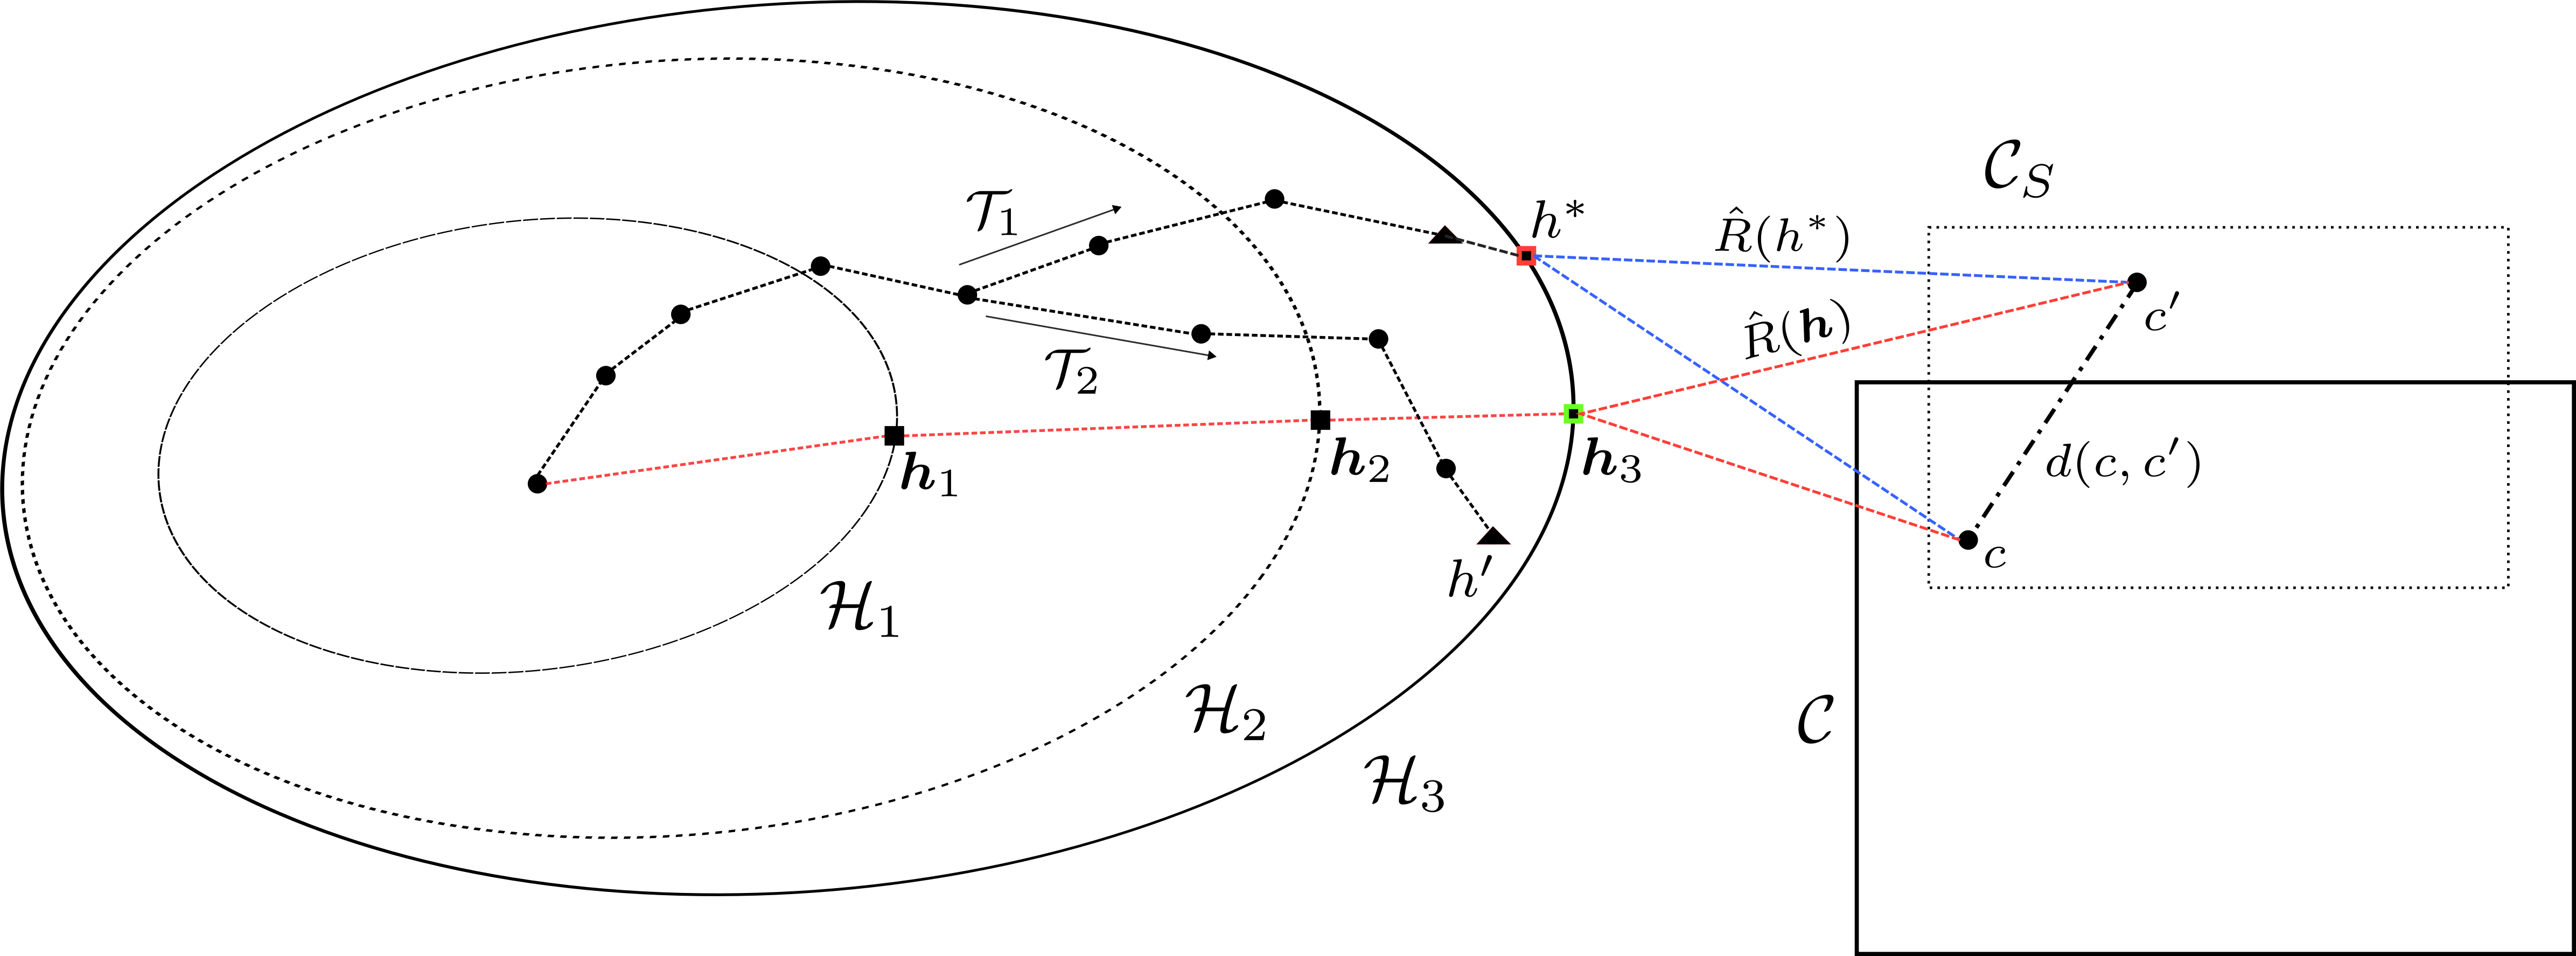
\includegraphics[width=0.7\textwidth]{media/g10.png}
  \caption{{\small \textbf{Illustrative dynamic of the learning problem.} For an incremental hypothesis space sequence $\mathcal{H}_{1},\mathcal{H}_{2},\mathcal{H}_{3}$, we aim to obtain the procedure $\mathcal{T}$ that would either reach the \textit{generalization solution} $\bm{h}$, or the \textit{empirical solution} $h^{*}$ for a particular hypothesis class, with respect to the concept $c$ and its observed concept $c'$. Model selection hence dictates how an algorithm or procedure than choose the best possible hypothesis to approximate the generalization solution from the empirical solution set. Do notice that here we explicitly state that the data would create a \textbf{proxy concept} that overlaps with the concept class and of some arbitrary `distance' from the true concept by $d(c,c')$. In case the two classes overlap, there still exists the arbitrary distance. Also, we can also observe the intuitive notion of increasing hypothesis class - while it indeed can help in getting closer to the concept class, the somewhat intrinsic property of current learning theory being the relative random procedure class make it probabilistically unstable.}}
  \label{fig:statlearnclassical}
\end{figure*}
For fixed $\mathcal{H}$, for fixed and sufficiently large $\mathcal{S}$, and no observation (data) errors, the empirical risk is the generalization risk. These two measures between $h$ and $c$ constitute the learning problem, which can also be separated into both cases - either empirical learning or generalization learning, one to minimize $\hat{R}(h)$, and one to minimize $R(h)$. Here, we emphasize such hierarchy by defining the generalization goal as the \textbf{nested criteria} for empirical risks minimization. 

\begin{definition}[Empirical learning problem]
    We present the formal form of the empirical learning. Suppose we have a \textbf{target}, $c\in\mathcal{C}$, where $\mathcal{C}$ is an arbitrary concept class that captures targets of the same type. Suppose we are provided a set of observations $\mathcal{S}$. The problem is to use certain algorithm $\mathcal{A}$ using $\mathcal{S}$, to obtain a hypothesis $h^{*}$ for a fixed $\mathcal{H}$ such that: 
    \begin{equation}\label{eq:lp1}
        R(h^{*}) = \min_{h\in\mathcal{H}} \hat{R}(h) = \min_{h\in\mathcal{H}} \underset{x\sim\mathcal{D}, x\in \mathcal{S}}{\mathbb{E}}\:\ell\{h(x),c(x)\}
    \end{equation} 
\end{definition}

The generalization best $\bm{h}$ is also called in literature as the \textit{Bayes model}, such that it reduces the Bayes risk that is the infimum of the generalization risk, $R^{*}=\inf_{h\in \mathcal{H}}R(h)$. The hypothesis $h^{*}$ is often called the \textit{empirical best}, for it being the minimal, finite hypothesis of the lowest loss evaluation on the entire observation space $\mathcal{S}$. There exists no certified assumption regarding whether $h^{*}$ aligns with the minimal generalization error.

\begin{definition}[Generalization learning problem]
    We present the formal form of the generalization learning problem. Suppose we have a \textbf{target}, $c\in\mathcal{C}$, where $\mathcal{C}$ is an arbitrary concept class that captures targets of the same type. Suppose we are provided a set of observations $\mathcal{S}$. Supposed we have an algorithm $\mathcal{A}$ that for fixed hypothesis space $\mathcal{H}$, \eqref{eq:lp1} holds true. The problem is to use certain algorithm $\mathcal{A}'$ such that, under limited availability, to obtain $\bm{h}$, satisfies: \begin{equation}
        R(\bm{h}) = \min_{h\in \mathcal{H}} R(\bm{h}) \leq \{\epsilon\}, \quad \epsilon > 0 
    \end{equation}
    For a set of risk bounds $\epsilon$. If the setting is deterministic, then there exists $\epsilon=0$ accordingly. 
\end{definition}

We can show that normally, the problem of empirical learning and generalization learning is not the same. That is, if one tries to solve the empirical learning problem to certain measure, then they will fail the generalization problem. This can be illustrated by figure \ref{fig:genvsemp_fig}. This problem between the disparity of the empirical and generalization target is what we often called as the \textit{Allegory of the cave}. This is the phenomena where we interpolate too much of the empirical space, when turning to the generalization space, the model instead is marginally significantly inaccurate. Here, we risk being dependent ourselves on false hypothesis obtained by empirical data acquisition, but also have to aim for the general form of the target by itself, which is often assumed unobtainable or impossible to know of prior belief. Hence, either that we take a skewed representation of reality through empirical data, or we diverge from such in a manner that gets closer to the ground truth's concept. At least in this setting, it is then observed as above that empirical learning problem is a subproblem toward generalization problem - one have to solve the empirical learning problem before attempting the generalization one. We also want to introduce the term \textbf{data shape} and \textbf{concept shape} for data $\mathcal{S}\in c$ and the shape of $c$ by itself, to reflect this difference. 

Further progression on such description for the process of generalization goal can be, realized in certain form as the global optimization objective in which empiricism can obtain from reasonable set of assumptions and conditions. The following algorithmic framing indeed aims to focus and extradite such sense of operational goal, where we directly attempt such. We note that the differentiable field $\nabla$ itself is a placeholder on similar-typed object, so as for us to not commit to any closure systems prematurely. 

\RestyleAlgo{ruled}
\SetKwComment{Comment}{}{}
\SetKwBlock{Objective}{Objective}{}
\begin{algorithm}[htb]
    \renewcommand{\algorithmcfname}{Optimization problem}
    \caption{Empirical-generalization learning dynamics (non-proxy)}
    \KwData{$(x_{i},y_{i})\in\mathcal{S}, \Gamma \supset \mathcal{S}$, objective $\ell(y,f(x))$, $\nabla(\cdot)$ differentiable gradient field on $\ell$.}
    \KwResult{Expected optimized model to the minimal error on the objective $\ell(\cdot,\cdot)$, dependent on $\mathcal{S}$.}
    \Begin
    {
        $\Gamma\supset \mathcal{S}$, the general set\;
        $R(\cdot),\hat{R}(\cdot)\gets\ell$ as objective functional\;
        \For{Fixed $\mathcal{H}$, with $h\in\mathcal{H}$, for $\epsilon > 0$}{
            Find $h\to \bm{h}'$, using algorithm $\mathcal{A}$ for minimization objective, such that 
            \begin{equation}
                \mathcal{A}\left(\min_{h\in\mathcal{H}} \hat{R}_{\mathcal{S}}(h) + R(h)\right) \leq \epsilon 
            \end{equation}for procedure $\mathcal{A}(\cdot,\cdot)$ of structural constraints.\;
        }
    }
    \Return{Optimized model $h$ on arbitrary objective space $(\ell,\nabla)$.}
    \label{algo:algo_optim_ideal}
\end{algorithm}

These two stages of learning procedure comes of as the intrinsic design of machine learning setting. As opposed to interpolation, where empirical learning problem would have to be put into first priority to achieve the best possible point-through model, machine learning leans on approximation more and a separated criterion that is only visible in the learning setting - the fact that we are using $c'$ to extract $c$. This disparity is exactly the \textbf{generalization problem}, of which is then also the goal of machine learning, to approximate the general solution using the observed solution. One then can ask what is the difference between the two notions, and when we can guarantee that both will `converge' to the same point. The process of \textbf{model selection} is then the procedure that will optimize $h\in \mathcal{H}$ to a given target fixture, such as the empirical best. 

One of the major assumption or observation from the point of the hypothesis class, is that the hypothesis cannot know the generalization error. Thereby, the more efficient and often used procedure/algorithm in training, is then the \textit{empirical risk minimization} (ERM) method, minimizing only the empirical risk to the empirical best; then, certain measures to `generalize' this heuristically is apprehended on the hypothesis. The process of model selection is also the place that we get the concept of \textbf{bias-variance tradeoff}, and its longstanding form to be a foundational metric on model selection. 

In general, to fit also the former theories, in the classical learning setting, we can dissect the problem into what constitute the following cleaner version of the setting, includes both the generalization learning and empirical learning problem. Again, under ideal condition, and ideal setup, the learning setting will have empirical learning and generalization learning to be on the same track. Later on, we would formalize what exactly on the same track means. 

\begin{setting}
    Given an op-space $\mathcal{X}\times\mathcal{Y}$, define the concept class $\mathcal{C}$ of all $c: \mathcal{P}(\mathcal{X})\to \mathcal{P}(\mathcal{Y})$ of all power set for both, where $\mathcal{X}\sim \mathcal{D}$ for some distribution $\mathcal{D}$ of the probabilistic assumption. The learning problem consists of defining a hypothesis class $\mathcal{H}$, for $h$ being an arbitrary hypothesis, either with specific architecture or not, and a learning algorithm $\mathcal{A}$, of a \textbf{learner} such that the following is acquired: 
    \begin{itemize}[itemsep=1pt,topsep=1pt]
        \item Set $\epsilon,\delta> 0$ be the error bound and the confidence measure (that is - the probability of failure) of $h$, for $\ell$ the evaluative measure of $\{h(x),c(x)\}$, define $\hat{R}(h)$ being the empirical risk of $h$ on the observation set $\mathcal{S}$ available. Then, the \textit{empirical learning problem} is tasked to find the hypothesis such that $\hat{R}(h) = \min_{h_{0}\in \mathcal{H}}\hat{R}(h_{0})\leq \epsilon$ for some arbitrary $h_{0}$, with confidence $1-\delta$. This $h$ is called the \textit{empirical best}. 
        \item Similarly, define $R(h)$ the generalization error, assumed outside $\mathcal{S}$. Then, the \textit{generalization learning problem} is tasked to find the hypothesis such that $\hat{R}(h) = \min_{h_{0}\in \mathcal{H}}R(h_{0})\leq \epsilon$ for some arbitrary $h_{0}$, with confidence $1-\delta$. This $h$ is called the Bayes model. 
        \item The generalization setting requires choosing the optimal point for both $h^{*}$ of the empirical best, and $h_{B}$ for Bayes hypothesis. 
    \end{itemize} 
\end{setting}
To choose and to compare between the empirical best, and the generalization best, we need certain notions to compare the two, algorithm to choose and evaluate, and metric to determine how comparison should be performed, with both measurable. At best, we need to find the correlation between the subconcept and the actual target concept itself. 

\subsection{Overfitting and underfitting}

Following the above framework of statistical probabilistic learning theory, one understanding about the concept of underfitting and overfitting (similar to \cite{James2021}) can be reached, using the notion of \textit{partitioning} of observation space. Such work is typically done because of \textbf{practical condition}, in which the following constraints is applied.
\begin{assumption}\label{assume:cpi_transparency}
    No knowledge of $c\in\mathcal{C}$ is provided. Consequentially, $R(h)$ cannot be accessed for any particular $h$ \footnote{Few points need to be said about this assumption. This assumption represents the \textit{worst-case possible} of a system dynamic. From the perspective of a designer, inherent leakage of information can be provided in the design of a model. In such, case we are operating in the mode of a \textit{resource-constrained, closed} game, in which the model with further assumptions of fixed class, operates on. The problem space itself is inherently large and penalize any additional structural changes. If one is to occur, we usually mention it as \textit{implicit bias}, but another name that would be more fitting would be \textit{structural attractor}, after the notion of gradient attractor in chaotic systems.}.
\end{assumption}

Without such knowledge, $R(h)$ cannot be computed, accordingly, and so under circumstances, it can only satisfy the empirical risk notion if one is to procedurally ignore generalization possibiities. We specify such approach as \textit{heuristic}, as it is only an approximation, and for better definition, we define it as followed. 

\begin{definition}[Heuristic empirical risk]
  Given a dataset $\mathcal{S}$ of size $m$, supposedly of the concept $c\in \mathcal{C}$, and the hypothesis $h\in \mathcal{H}$, then the \textbf{heuristic empirical risk} take a partitioning $k<m$ with $k/m\geq 1/2$, hence defining the heuristic empirical loss on $k$, denoted $\hat{R}_{k}(h)$. 
\end{definition}

\begin{definition}[Heuristical generalization risk]
  Given a dataset $\mathcal{S}$ of size $m$, supposedly of the concept $c\in \mathcal{C}$, and the hypothesis $h\in \mathcal{H}$. Fixed $\hat{R}_{k}(h)$, for the final optimization of algorithm $\mathcal{A}$, then the \textbf{heuristic generalization risk} take the remaining 2-partition of portion $p=k-m$, hence defining the heuristic generalization loss on $p$, denoted $\hat{R}_{p}(h_{\mathcal{A}})$. 
\end{definition}
The two heuristic definition however, can be noted to not be equal to the true generalization risk - empirical risk pair in reality. Nevertheless, one can then define overfitting and underfitting in such manner. 
\begin{definition}[Underfitting]
  A model $h$ is called \textbf{underfitting} if for a constant $\epsilon > 0$ chosen for the setting, then $\hat{R}_{k}(h_{\mathcal{A}})>\epsilon$, $\hat{R}_{p}(h_{\alpha})> \epsilon$ over the entire observation space. 
\end{definition}
Usually, underfitting is defined to be such that test error is smaller than training error partition, however, we do not think that is a good definition. Especially since, at least in this setting, the empirical error under algorithm $\mathcal{A}$ is reduced to the representative smallest error that $\mathcal{A}$ can achieve on that particular model, within particular setting of $h$, then come the heuristic generalization error. Considering also that $k/m\geq 1/2$, that is, at least the training partition is half of the observation set, then only under very specific case will $\hat{R}_{p}(h_{\alpha})$ be smaller than $\hat{R}_{k}(h)$, statistically speaking. Thence this line of thought also reinforces the idea that both of them will be larger than the threshold $\epsilon$. Usually, heuristically, this threshold of error is $0.3$, normalized. Next, we define the notion of overfitting. 

\begin{definition}[Overfitting]
  A model $h$ is called \textbf{overfitting} if there exists a specific constant $\epsilon>0$ chosen for the setting, such that $\hat{R}_{k}(h)<\epsilon$, $\hat{R}_{p}(h_{\alpha})> \epsilon$ over the entire observation space.
\end{definition}
Namely, this mean that the static learning makes the generalization error worse. This draws the analogy of the student - studying explicitly for the past paper tests, yet unaware of the larger margin of questions in the large set of the test paper pool, leading to subpar performance. Similarly, overfitting is theorized to be fitting too fit to the reduced observation space - hence when it comes to the generalization observation space, it fails within such heuristic. The notion works on the mask of the risks, $\hat{R}_{k}$ and $\hat{R}_{p}(h_{\alpha})$. 

In practice, Assumption~\ref{assume:cpi_transparency} means we cannot have $c\in\mathcal{C}$, or its probabilistic interpretation $\mathcal{D}$ such that $x\sim\mathcal{D}$, or in the extreme non-structured case, $(x,y)\sim \mathcal{D}$. In such case, the typical practical fix relies on the partitioning of the available partitioning space, that is, the empirical-generalization proxy. For large enough singleton count of $|\{(X_{k},Y_{k})\}|$, we assume that $\hat{R}_{\mathsf{Gen}}(h)\approx R(h)$. Thus, the algorithm can be stated in a form as Algorithm~\ref{algo:algo_optim_no_c}.

\RestyleAlgo{ruled}
\SetKwComment{Comment}{}{}
\SetKwBlock{Objective}{Objective}{}
\begin{algorithm}[htb]
    \renewcommand{\algorithmcfname}{Optimization problem}
    \caption{Empirical-generalization learning dynamics (proxy)}
    \KwData{$(x_{i},y_{i})\in\mathcal{S}, y_{i}=\{\pm 1\}$, hinge objective $\ell(y,f(x))$, $\nabla(\cdot)$ differentiable gradient field on $\ell$.}
    \KwResult{Expected optimized model to the minimal error on the objective $\ell(\cdot,\cdot)$, dependent on $\mathcal{S}$.}
    \Begin
    {
        $((X_{1},Y_{1}),\dots)_{n}\gets\mathsf{Partition}_{n}(\mathcal{S})$\;
        $\{(X_{j},Y_{j})\}\gets \mathsf{Train}$\;
        $\{(X_{k},Y_{k})\}\gets \mathsf{Gen}$ for $k\ne j$\;
        \For{Fixed $\mathcal{H}$, with $h\in\mathcal{H}$, for $\epsilon > 0$}{
            (Optimistically) achieve $h\to \bm{h}'$, using algorithm $\mathcal{A}$ for minimization objective, such that 
            \begin{equation}
                \mathcal{A}\left(\min_{h\in\mathcal{H}} \hat{R}_{\mathsf{Train}}(h) + \hat{R}_{\mathsf{Gen}}(h)\right) \leq \epsilon 
            \end{equation}for procedure $\mathcal{A}(\cdot,\cdot)$ of structural constraints.\;
        }
    }
    \Return{Optimized model $h_{\mathcal{A}}$ on arbitrary objective space $(\ell,\nabla)$.}
    \label{algo:algo_optim_no_c}
\end{algorithm}
The assumption above of the generalization set to the generalization truth error is apparent in the usual system theorem, Theorem~\ref{thm:minimalNeu}.
\begin{theorem}[\cite{10.5555/2371238}]\label{thm:minimalNeu}
    For fixed $\mathcal{H}$, for fixed and sufficiently large $\mathcal{S}$, and no observation errors, the empirical risk is the generalization risk: \begin{equation}
        \underset{\mathcal{S}\sim \mathcal{D}^{m}}{\mathbb{E}}[\hat{R}_{\mathcal{S}}(h)]  = R(h)
    \end{equation} 
\end{theorem}

\begin{proof}
    By linearity of the expectation, and the fact that we assume the sample is given i.i.d., we can write: 
\begin{equation}
    \begin{split}
        \underset{S \sim \mathcal{D}^m}{\mathbb{E}}[\hat{R}_S(h)] 
        &= \frac{1}{m} \sum_{i=1}^m 
            \underset{S \sim \mathcal{D}^m}{\mathbb{E}} 
                    \left[ \mathbbm{1}_{h(x_i) \ne c(x_i)} \right] \\
        &= \frac{1}{m} \sum_{i=1}^m 
            \underset{S \sim \mathcal{D}^m}{\mathbb{E}} 
                \left[ \mathbbm{1}_{h(x) \ne c(x)} \right], \\
    \end{split}
\end{equation}
for any \( x \) in sample \( S \). Thus, we result in

\begin{equation}
    \begin{split}
        \underset{S \sim \mathcal{D}^m}{\mathbb{E}}[\hat{R}_S(h)] 
            &= \underset{S \sim \mathcal{D}^m}{\mathbb{E}} 
            \left[ \mathbbm{1}_{h(x) \ne c(x)} \right] \\
            &= \underset{x \sim \mathcal{D}}{\mathbb{E}} 
            \left[ \mathbbm{1}_{h(x) \ne c(x)} \right] \\
            &= R(h).
    \end{split}
\end{equation}
which yields the desired result. 
\end{proof}

This theorem can be transferred to a more generalized conjecture, of which fit the generalized notion of the empirical proxy and so on. 
\begin{conjecture}
    Supposed $\mathcal{H},\mathcal{C}$ are fixed, for $\mathcal{S}$ is the empirical $c^{*}$ for $c\in \mathcal{C}$ the true concept. Then, for algorithm $\mathcal{A}(\cdot,\cdot)$ enforcing minimization apparatus, and the specific objective on the second argument, we have:
    \begin{equation}
        \begin{split}
            &\underset{j\to\infty,\mathcal{S}_{i}\neq\mathcal{S}_{k}}{\mathcal{A}}\left(\min_{h\in\mathcal{H}} \hat{R}_{\mathsf{Train}}(h) + \hat{R}_{\mathsf{Gen}}(h), [\ell]\right)\\
            & \quad \quad \approx \mathcal{A}\left(\min_{h\in\mathcal{H}} \hat{R}_{\mathcal{S}}(h) + R(h), [\ell]\right) + \epsilon_{\mathcal{S}}
        \end{split}
    \end{equation}
    For $\mathcal{S}_{i}\neq\mathcal{S}_{j}$ such that there are only distinct samples, $j$ the observation set size, $[\ell]$ the set of structural or empirical objectives enforced on the problem landscape, and $\epsilon_{\mathcal{S}}$ is the empirical minimum that the algorithm result can achieve assuming sufficient `perfect interpolation'. 
\end{conjecture}

By the end of this section, we would also want to note that we deliberately choose an expression basis of $\mathcal{A}$ via the couple tuplet $(\min, [\ell])$ as a choice for \textit{algorithm-agnostic class} of algorithm satisfies the dynamic only, not just implementations. The algorithm, in certain sense, depends much more on structural assumptions, of which is not accessible via observations but via design, and intrinsic information specified in the observation class itself. This is a requirement for fine-tuning analysis in the long-run, as there exists a myriad of different approaches. Indeed, the classical theory of learning simply does not have much to offer in terms of a unified perspective, in which important factors are analysed of its realization. Specifically speaking of such, classical theory does do worse in many parts, for example, the aspect of transparency given the model, supervisor and the concept, of which their roles are not fully understood or formulated correctly, both in controlled setting and extension to replication of real life examples. Thereby, the problem requires a newer theory of learning to come forward. A new learning theory must extend beyond what constitute the basic learning model, such as the idealized PAC-learning, and statistical learning setting in general. More specifically, we want to design a learning theory that is more akin to \textbf{modelling theory} of its internalization, but also attain the learning of machine learning theory. 

Within the constraints of such theoretical framing, we can then construct a different notion in which the generalization and the empirical learning problem can possibly relate to each other, at least from the statistical framework. Let us consider the problem of mathematical modelling in such sense. Beside the model class construction, which will be discussed in further sections, the entire idea of this structuralization is to refine the framework of which learning and so on can be defined itself. 

\section{System-wide structuralization}

From which we can draw out of the above discussions, concurrent theories are inherently unstable and with many variations, making them ill-suited for instant application on analysis of different models without losing major information about the structural details and expressions. Hence, we propose a novel analysis on the basis of the axiomatization of the learning setting, under various structural assumptions, which lies in the implementation sections. For now, we defer to the insight in which justify such movements. 

\subsection{The idea of neural network formalism}
Previously, we have been discovering, examining past results and testing on models of different types, generally classical models. While decisive, each modelling setting requires different analysis and is often not so streamline, typically fragmented as per different functional schemes, probabilistic schemes, optimization and algorithmic-based choice of designs, and so on. They have barely any unified view or general patterns for extension, thus making analysis inherently difficult. Within such, our interest, and discovery, posit that the formalism or the idea of neural network (accordance to designs and patterns of \cite{mcculloch_pitts_1943,hebb_1949,rosenblatt_1958,widrow_hoff_1960_adaline,minsky_papert_1969,fukushima_1980,kohonen_1982,hopfield_1982,werbos_1974,rumelhart_hinton_williams_1986,cybenko_1989,hornik_1991,hochreiter_schmidhuber_1997,lecun_bottou_bengio_haffner_1998,bishop_1995,haykin_1994}) and some of its modern understanding (as of \cite{goodfellow2016deep,zhang2023mathematical,hinton_osindero_teh_2006,lecun_bengio_hinton_2015,goodfellow_et_al_2014,srivastava_hinton_2014_dropout,szegedy_2014_inception,simonyan_zisserman_2014_vgg,vaswani_et_al_2017_transformer,he_zhang_ren_sun_2016_resnet,devlin_2018_bert,brown_et_al_2020_gpt3}) practiced and exhibited, to be, in its general form, the correct but ill-defined and poorly developed framework. Thus is our goal in this section to layout such task, and the development that will be described in this section. 

\subsubsection{Basic understanding}

In modern form, a neural network (\cite{goodfellow2016deep,zhang2023mathematical}) $N$ is typically specified by the dual $(L,[S])$ where $L$ is the number of processing layer of a neuron, and $[S]$ is the list of neurons configuration per layer - for example, the number of neurons per layer, and so on. For such network, the definition can be simple as followed 

\begin{definition}[Standard multilayer network, \cite{zhang2023mathematical}]
    We define a $K$-layer fully-connected deep neural network with real-valued output. Let $m^{(0)}=d$ and $m^{(K)}=1$ for $m$ the width of the network, and $d$ the shape of the input vector. We then recursively define: 
\begin{align}
    x_{j}^{(0)} &= x_{j} \quad (j=1,\dots,m^{(0)}),\\ 
    x_{j}^{(k)} &= h\left(\sum^{m^{(k-1)}}_{j'=1} \theta_{j,j'}^{(k)}x_{j'}^{(k-1)}+ b_{j}^{(k)}\right)\quad (j=1,\dots,m^{(k)}),\\
    f(x) & = x_{1}^{(K)} = \sum^{m^{(K-1)}}_{j=1} u_{j}x_{j}^{(K-1)}
\end{align}
where $k = 1,2,\dots,K-1$, for the model parameters can be represented by $w=\{[u_{j}, \theta_{j,j'}^{(k)}, b_{j}^{(k)}]: j,j',k\}$ with $m^{(k)}$ being the number of hidden units at layer $k$; $\theta\in \mathbb{R}^{m}$ the weight of the neuron.
\end{definition}

Here, each neuron is denoted by their expression as $f(\mathbf{W}^{\top}\mathbf{x}+b)$ for the activation function $f$. We can simplify a lot of those structures above into the neural network schemes. For example, the linear function class case can be simplified to a single $(2,[n,1])$ neural network, such as: 
\begin{align}
    x^{(0)}_{j} &= x_{j} \quad (j=1,\dots,n)\\
    x^{(1)} &= \sum_{j'=1}^{n} w_{j'}x_{j'}, 
\end{align}
without the activation function $h$. The polynomial neural network can be represented by simply a shallow, $[3,p]$ neural network. More concretely, if we take the \textit{input channel} as a (pre-)layer, then
\begin{align}
    x_{j}^{(0)} &= x_{j} \quad (j=1,\dots,m^{(0)}),\\ 
    x_{j}^{(1)} &= h\left(\sum^{m^{(0)}}_{j'=1} \theta_{j,j'}^{(1)}x_{j'}^{(0)} \right)+b_{j}^{(k)}\quad (j=1,\dots,m^{(1)}),\quad h(x_{j})=x^{j}\\
    f(x) & = x_{1}^{(2)} = \sum^{m^{(1)}}_{j=1} u_{j}x_{j}^{(1)}
\end{align}
for a neural network of shape $(3,[n,n,1])$, and of polynomial custom scaling function. For support vector machine, this is even harder to do, since its definition varies between different notion of the model itself. However, it is interesting because we can treat it as an arbitrary generation of a neural network structure. There are papers about formalizing SVM in the sense of neural network, including making it to be an infinitely-wide shallow neural network, for example, \cite{chen2021equivalence,wang2019svmdsn,zhang2014equivalence}, however, the structure that is formed from the SVM learner can be expressed as followed:

\begin{setting}[Support vector machine]
    For any given optimization problem on input space $x_{i}\in \mathbb{R}^{d}$, and label $y_{i}=\{\pm 1\}$, the shallow neural network resultant from the training procedure is always of the form:
    \begin{align}
        x_{j}^{(0)} &= x_{j} \quad (j=1,\dots,m^{(0)}),\\ 
        x_{j}^{(1)} &= \sum_{j'\in m^{(1)}} \theta^{(1)}x_{j'}^{(0)}K(x_{j'}^{(0)},x)\\
        f(x) & = \sign{(x_{1}^{(2)}) }
    \end{align}
    for a specific kernel $K(x,x')$. 
\end{setting}

Those three fundamental conversions to neural network raise interesting insight into the neural network formalism. For linear and polynomial shallow neural network, we design the network and then provide it with a training scenario, evaluated of the proxy generalization. SVM however can be considered an adaptive data construction, where the neural network is constructed from the dataset or observation set itself, using minimization on RKHS and with constraints. This prompts exactly as such, on one side the pre-optimization construction, and one is the post-construction optimization of a neural network architecture. This interpretation is surprisingly useful when talking about neural network's unit-like structure. Hence, from such evidence prompts us to analyse a neural network, not in only the sense of managing its layers, but also by its unit components together. 

This way of analysing unit-wise gives us much more interpretability, and also potential for a newer kind of network specification. As far as we are concerned of, a neural network can represent an active \textit{mathematical modelling system}. This then indicates, for example in adversarial learning case between the target neural network tailored to specific concept, and the learning hypothesis network, then the process of learning itself can be loosely interpreted as a concept of mathematical modelling representation learning, even in the case of black-box model, and not just simply phenomenological modelling of statistical data. To do this, we will examine the structure from the perspective of a \textbf{generator}.

\subsubsection{The SVM generator}

Support vector machine, first formally originated from \cite{Vapnik1999-VAPTNO}, is a model inherently, specifically defined for pattern recognition task, and binary classification via an \textit{optimal separating hyperplane}. There are two variants for SVM, namely, for linear and nonlinear hyperplane, but the main general aspect of SVM is its reversal of the direction on model building - instead, it aims to minimize the structure of a model, using the data-dependent structure, or \textit{support vectors}. 

The SV machine implements the following two precursor ideas: It maps the input vectors $x$, supposed of the setting, into a high-dimensional feature space $Z$ through some nonlinear mapping, chosen a priori. In this space, an optimal separating hyperplane is constructed. By statistical learning theory, Vapnik restricted the function class (as for infinite hypothesis it is impossible to learn) to the class of hyperplanes by 
\begin{equation}
    \langle \mathbf{w}\cdot \mathbf{x} \rangle + b = 0 ; \quad \mathbf{w}\in \mathbb{R}^{n} , b\in \mathbb{R}
\end{equation}
which $\mathbf{w}$ is the controlling weight, $\mathbf{x}$ is the input space to the space of all binary $\{-1,+1\}$ category. Hence, this basically divide the input space into two: one part containing vectors of the class $-1$ and the others being $+1$. If there exists such a thing, then it is said to be \textit{linearly separable}. To find the class of a particular vector $\mathbf{x}$, we use the following decision function 
\begin{equation}
    f(\mathbf{x}) = \mathrm{sgn}[\langle \mathbf{w}\cdot \mathbf{x}\rangle+ b]
\end{equation}
This is called the \textbf{hyperplane classifier} class\footnote{As can be understood simply from such, there exists many hyperplanes that can correctly classifies the classes. It has been then shown that the hyperplane that guarantees the best generalization problem performances is the one with the maximal margin of separation between two classes (\cite{Cristianini2000AnIT}).}. The above form of finding final classification can then be presented in dual form, which then depends only on dot products between vectors, as 
\begin{equation}
    f(\mathbf{x}) = \mathrm{sgn}\left(\sum^{\ell}_{i=1} y_{i}\alpha_{i} \langle \mathbf{x}\cdot \mathbf{x}_{i} \rangle+ b\right)
\end{equation} 

where $\alpha_{i}\in \mathbb{R}$ is a real-valued variable that can be viewed as a \textit{measure} of how much informational value $\mathbf{x}_{i}$ has (for $x_{i}$ the support vectors we get from training)\footnote{The \textit{support vector} of a particular hyperplane $\mathbf{y}$ is the collections of all points that lies closest to the hyperplane, which is specified as condition for maximization on both side of maximal margin vector machine.} The second idea is of the \textit{kernel method}. This particular method, useful and well-known of the time SVM was created, gain a more prominent position among other techniques, including neural network. Specifically, this method is characterized by the mapping of the input vectors into a richer (usually high-dimensional) feature space where they satisfy \textit{linear separable} criteria. This prompted the possibility to solve nonlinear problem through such mapping, and indeed yields a nonlinear decision surface in the input space, which is linear in the feature space. A \textbf{kernel} (function) is then a function $k(\mathbf{x},\mathbf{y})$ that given two vectors in input space, return the dot product of their images in feature space such that $k(\mathbf{x},\mathbf{y})=\langle \phi(x), \phi(y) \rangle$ for the nonlinear mapping $\phi$. The general form of SVM is then usually cited as 

\begin{equation}
    f(\mathbf{x}) = \mathrm{sgn} \left(\sum^{\ell}_{i=1} y_{i}\alpha_{i}k\langle \mathbf{x}\cdot \mathbf{x}_{i} \rangle\right)\quad \ell \leq n
\end{equation}
for any particular final categorization. One of the major problem for analysing SVM, is in the properties of it potentially having infinitely many parameters, depends on the size of the dataset. This makes the curve of both bias-variance and double descent not applicable in such regard - infinitely many parameters' complexity, yet still finite complexity class\footnote{From such observation, it would seem imperative that the notion of complexity based solely on the parameter counts of certain model construction is ill-equipped for certain flavours of machine learning model, in this case support vector machine (in the same type is the Gaussian Mixture Model). No double descent has been observed by empirical reports record per the author's knowledge.}. 

With respect to the observable space, SVM and neural network, we can call the construction scheme of SVM a type of \textit{backward construction} from data $\mathcal{S}$. Or rather, the following algorithm represents SVM construction problem: 

\RestyleAlgo{ruled}
\SetKwComment{Comment}{}{}
\SetKwBlock{Objective}{Objective}{}
\begin{algorithm}[htb]
    \renewcommand{\algorithmcfname}{Factory}
    \caption{Support Vector Machine - backward construction.}
    \KwData{$(x_{i},y_{i})\in\mathcal{S}, y_{i}=\{\pm 1\}$, hinge objective $\ell(y,f(x))$, $\nabla(\cdot)$ differentiable gradient field on $\ell$.}
    \KwResult{Expected optimized model to the minimal error on the objective $\ell(\cdot,\cdot)$, dependent on $\mathcal{S}$.}
    \Begin
    {
        $d\gets \dim|\mathcal{S}|$\;
        $n\gets|\mathcal{S}|$\;
        $\ell(y,f(x))=\max(0,1-yf(x))$\;
        Kernalization $\phi:\mathbf{x}\to\mathbf{x}'$\;
        $f(\mathbf{x})\gets \mathbf{w}^{\top}\phi(\mathbf{x})+b$\;
        \Objective
        {
            Attain the minimization 
            \begin{equation}
                \min_{w,b\in f} \frac{1}{2}||w||^{2} + C \sum_{1\leq i\leq n}\ell(y_{i},f(x_{i}))
            \end{equation}
            Ideally for $y_{i}(\mathbf{w}^{\top}\phi(\mathbf{x}_i)+b)\geq 1, \: \forall i, y_{i}\in\mathcal{S}$, penalized by $\ell$.\;
        }
    }
    \Return{Optimized model $\mathsf{SVM}(f)$ on objective $\ell$ of $\nabla$ field.}
    \label{algo:algo_SVM_no_kernel}
\end{algorithm}

Such a factory is reversed inherently, and with its formulation constrained in the form $\mathbf{w}^{\top}\phi(\mathbf{x})+b$, of which is equivalent to a non-linear shallow neural network with infinite width (\cite{wang2017research,chen2021equivalence}), but is not a full-fledged neural network in technicality, hence it is only a functional equivalence. That is, such result only indicates that for $N\to \infty$ of the number of neurons of a single-hidden layer neural network, $\sum_{j=1}^{N}a_{j}(w_{j}^{\top}x+b_{j})$, then 
\begin{equation}
    \mathsf{NN}(x) \approx \mathsf{SVM}(x) = \sum^{\ell}_{i}\alpha_{i}k\langle x,x_{i}\rangle, \ell \leq n
\end{equation}
The support vector, $\ell$ list, is inherently implicit of the factory itself. On the other hand, typical deep learning or neural network constructions are rather \textit{forward-constructed}, that is, the model is in a sense, prefabricated then tested of its efficacy, and thus the effective performance of the model is limited by iterations of its restricted frame. We can easily visualize the factory of which neural network are constructed, different of the SVM factory case: 

\begin{algorithm}[htb]
    \renewcommand{\algorithmcfname}{Factory}
    \caption{Neural Network - forward construction class}
    \KwData{$(x_i, y_i) \in \mathcal{S}$, loss $\ell(y, f(x))$, 
    $\nabla(\cdot)$ differentiable gradient field on $\ell$.}
    \KwResult{Optimized model on objective $\ell(\cdot,\cdot)$, 
    dependent on prefabricated $[\mathcal{H}]$.}
    \Begin
    {
        $d \gets \dim|\mathcal{S}|$\;
        $n \gets |\mathcal{S}|$\;
        Fix architecture $[\mathcal{H}]: \{L, \{d_l\}_{l=1}^L, \sigma\}$\;
        Initialize $\theta_0 \sim p(\theta)$ on $[\mathcal{H}]$\;
        $f(\mathbf{x}) \gets \sigma_L(W_L \cdots \sigma_1(W_1 \mathbf{x} + b_1) \cdots + b_L)$\;
        \Objective
        {
            Attain the minimization
            \begin{equation}
                \min_{\theta \in [\mathcal{H}]} 
                \frac{1}{n}\sum_{i=1}^{n} 
                \ell(y_i, f_\theta(x_i)) + 
                \lambda \Omega(\theta)
            \end{equation}
            via iterative $\nabla$-field update
            $\theta_{t+1} \gets \theta_t - \eta_t \nabla_\theta \ell$\;
            until $t \leq N$ or 
            $\ell[h_{M,N}] \leq \epsilon$\;
        }
    }
    \Return{Optimized model $\mathsf{NN}(f_\theta)$ 
    on objective $\ell$ of $\nabla$ field.}
\end{algorithm}

The difference is deliberate. 

\subsection{Attractor-based insights}

The above reformulation in this chapter, giving insights of the learning formulation typically observed, arguably still attains a lot of assumptions, of which we settle for the next section. Optimization procedure~\ref{algo:algo_optim_ideal} and procedure~\ref{algo:algo_optim_no_c} define the precursor tradeoff in the problem space, or rather, the heuristic-generalization tradeoff. We can state it as the following to clarify such problem in plain sight. 

\begin{theorem}[Heuristic-generalization tradeoff, model selection]
    An algorithm $\mathcal{A}$ on the system $(\mathcal{H},\mathcal{C},\mathcal{A})$, for the expected empirical heuristic $\hat{R}_{\mathsf{Train}}(h)$ and generalization heuristic $\hat{R}_{\mathsf{Gen}}(h)$ on $\mathcal{S}$, on the measure landscape of $\mathcal{L}[\ell]$ for $\hat{R}(\cdot)$, of which $\mathcal{A}$ runs separately on $\mathcal{A}'(\mathsf{Train},h)$ and $\mathcal{A}'(\mathsf{Gen},h)$ for the above heuristic, there exists \begin{equation}
        \left\{ \underset{h\in \mathcal{H}}{\argmin}\:\hat{R}_{\mathsf{Train}}(h), \underset{h\in \mathcal{H}}{\argmin}\:\hat{R}_{\mathsf{Gen}}(h)\right\}\in \mathcal{L}[\ell]
    \end{equation}
    as \textbf{convex attractor} on the measure landscape. Then, algorithm $\mathcal{A}$ \textbf{solves} the generalization if for the transition $\mathcal{T}:\mathcal{L}_{\mathsf{Train}}[\ell]\to\mathcal{L}_{\mathsf{Gen}}[\ell]$ for separated loss-landscape, it satisfies for $\mathcal{A}(\mathcal{S},h)\to h'$, that 
    \begin{equation}
        h' = \underset{h'\in \mathcal{H}}{\argmin}\: \left(\hat{R}_{\mathsf{Train}}(h) + \hat{R}_{\mathsf{Gen}}(h)\right)
    \end{equation}
\end{theorem}
This tradeoff relies on the precursor concept of the \textbf{attractor} landscape, of which is observable within the objective-space expansion from $\mathcal{L}_{\mathsf{Train}}[\ell]$ to $\mathcal{L}_{\mathsf{Gen}}[\ell]$ of the heuristic space. The partition $\{(X_{j},Y_{j})\}$ and $\{(X_{k},Y_{k})\}$ covers the practical notion of cross-validation, though the cross-validating procedure itself works much different, as it covers multiple re-shuffling, i.e. unordered re-partition of the default permutating groups. This is the theorem of purpose in which we are to prove. Such requires further clarification, and thus form the basis for this particular len. 

\section{Reattaching the neural perspective}

Since the previous analysis of the learning model, we can then notice a few disadvantages and a few very subtle points that we omitted. It is apparent that the analysis is somewhat entangled, with various situations, interpretations, setting and assumptions together, and with a non-unified structure of models in question. The system in which the model is considered and analysed is also missing in essence. There are a lot of ambiguities around what is considered and what is not, even with probabilistic nature and the deterministic aspect. Terms like \textbf{latent spaces} and many do not capture the entire dynamic or meaning of the system. It is then we introduce our novel analytical framework, namely the \textbf{Unified Unitary Construct} framework. It is however, can be said otherwise that the learning theory is rather not so novel, but approaching the problem is a more distinct way of the already existing framework. 
\section{Motivation}
The predecessors of neural network, for operations and purposes, take in the form of a specific application of function constructs, finite singleton algorithms. For such purposes, a specific classical model $m$ takes the form of a single structure, with complex construction, often offering fixed architecture of its representation. Neural network is an attempt, for its philosophy, to change the aforementioned philosophy of constructing machine model by considering compute unit \cite{mcculloch_logical_1943,Rosenblatt1958ThePA}. 

Motivated by earlier analysis and observations, it is apparent that the analysis is fragmented, with various situations, interpretations, setting and assumptions together, and with a non-unified structure of models in question. The system in which the model is considered and analysed is also ineffective when considering larger structures or more `realistic' consideration aside from very simplified, strong system itself. There are a lot of ambiguities around what is considered and what is not, even with probabilistic nature and the deterministic aspect. Terms like \textbf{latent spaces} and many do not capture the entire dynamic or meaning of the system. It is then we introduce our novel analytical framework, namely the \textbf{Unified Unitary Construct} framework. It is however, can be said otherwise that the learning theory is rather not so novel, but approaching the problem is a more distinct way of the already existing framework. 

Recalled the classical learning framework, for $h$. We know and construct the principle of the system by settle on $h:\mathcal{X}\to \mathcal{Y}$, for any arbitrary defined in-out 2-tuple. Hence, the overall construction of a given model can be abstracted into layers of responsive results. This in particular draws some advantages, for example, can be easily approximated or expressed in the black box model style, or empiricism approach. However, it also comes with the drawback that we have seen, in the sense that the interpretation of such black box model is very narrow, even after we add different kind of flavours, for example, the assumptions of the Gaussian noise. This is majorly because of applying and addition of different components without a general framework, leading to a lot of messiness when looking directly into the theory itself. Specifically, for example, is the fact that there exists two kinds of learning analysis, one considers the information-theoretic approach of information exchange, while the other is simply the classical approach given in such the intrinsic noise error given by the observation set itself, keeping the classical theory intact. How to formalise this is a big hurdle to incorporate each other in, without considering the wider framework - one of the main problem with the speciality of learning theory. Nevertheless, at least accordance to general theory of the current date, formalization in to unit-like processing unit as \textit{neural network components} is one thing that should be considered for the learning framework. This is also one of the main point for the word \textbf{Unified} in our theory. 


%\subsection{Probability}
%
%Probability is a loose concept, most generally speaking. Usually, it refers to the uncertainty in our action, hence %taken of virtue of subjectivity given certainty being not absolute. As reconciled by \cite{Nau2001_DeFinettiWasRight,%deFinetti1990_TheoryProbability,Elliot2019_DeFinettiPhilosophy}, probability can be described to be of the \textit%{degree of belief} of certain agent abstraction - an object or specimen that receives and act on the environment it %beholds. In such sense, we can also interpret our system to explain the uncertainty that unfolds. 
%
%Taken as an observer tasked with predicting and interpreting the system $\mathcal{S}_{0}$, then, by the standard %definition of ambiance space. A system that is \textit{total predictable} and \textit{deterministic} if, the encoding %space is empty, $\mathcal{E}=\varnothing$, and $\mathcal{L}^{*}=\mathcal{L}_{E}$. What this means is that all %descriptions are known, the language is observable from such, and there are no encoding. This is the \textit{ideal %system}. 

%\subsection{The concept of learning}
%
%Within the authoritative sources on the modern deep learning theory, like \cite{neyshabur2015norm,neyshabur2017exploring,NJacot:2018:NTK,arora2019finegrained,lee2019wide,chizat2019lazy,zou2019implicit,bartlett2021deep,roberts2022principles,wei2022theory,yang2019scaling} in comparison, the new theory of modern networks, or deep learning, remains a very troublesome regime with a lot of unspecified behaviours or outcomes leading on its structures. Unsolved problems emerged from the structural usage, for example, double descent, grokking, neural scaling limits, etc, all of which hinders and expose the immaturity of the concurrent theory. As such, a direction to take on to resolve such issue must be contained, effectively nonetheless. 

\subsection{Neurons perspective}

The formalization to be \textit{atoms} comes from the biological inspiration of exactly the biological neurons in human and species' brain. However, the mechanism and how they operate is a bit more interesting. 

For the biological more advanced equivalent, the brain consists of a very large number of highly connected elements, called \textit{neurons}. The simplified structure of such neuron consists of three components: the \textit{dendrite}, which is tree-like receptive network that carry signals (electrical) to the cell body; the \textit{cell body} effectively processes these signals, usually as sums and threshold response; and the \textit{axon}, a single long fibre that carries signal from the cell body to other neurons. The point of contact between an axon and a dendrite of another cell is called a synapse. The neural network, hence, is established by the synapses and various arrangements of the neuron. 

This configuration of biological neuron is particularly powerful. Not only that they can process information allowing someone to write this text, but also the fact that of billions or neuron, they parallelly work at the same time. Furthermore, the intricacy lies further ahead than the above formation - the entire structure is of too much complexity, for the brain itself. However, a principle can be seen - they are contained of \textit{building blocks} together, in which case is neuron. And \textbf{artificial networks} also take this approach. 

\begin{note}
From such, we can conclude that, we have to have some classification that requires the smallest component neuron to be the \textit{atoms} that everything else is formed upon.
\end{note}

One of the most fundamental thing of the structure of the \textit{neural network formalism}, hence, is the notion of a \textit{unit neuron}. Specifically, a neuron $x$ is defined, and designed to be a discrete operating unit on its own. The word \textit{operating} here means that it has all the facility requires for an input-output process - the most simple one includes the input receiver, the processing formulae, and the output transmitter. 

The neural network formalism is best expressed by the following principle. This theorem is by design, and thus our design is to fix the foundational minimization to a specific neuronal basis module. Such is to say, we state the principle for \textit{inductive recursion} of neuronal system collapse. 

\begin{theorem}[Fundamental theorem of neural formalism]\label{thm:fundamental_neuron}
Let $\mathcal{S}$ be an automated operational system with internal composition system, admitting
\begin{enumerate}[topsep=1pt,itemsep=1pt]
    \item nontrivial input-output interaction,
    \item internal closure under composition, and
    \item irreducibility with respect to its operational primitives.
\end{enumerate}
Then any minimal operational component of $\mathcal{S}$ must admit a representation whose cardinality and arbitrary (analytic, topological, etc.) structures are equivalent to that of the minimally defined neural structure $\mathfrak{N}(\mathcal{N},\mathcal{C})$.
\end{theorem}

We begin by examining the model of a typical neuron. Note that, this is the simplest one, but also is the fundamental block. We have the following. 

\begin{definition}[Neuron]
    Given the neural network formalism. Define a construct $x$. Then $x$ is called a \textbf{neuron} if it belongs component-wise to the class $\mathcal{N}$ of all neurons, which is minimally expressed by $\mathcal{N}(n_{i},n_{o},M(\dots))$, where $n_{i}$ is the input handler, $n_{o}$ is the output handler, and $M(\dots)$ is the internal system. %\index{classical neuron}
\end{definition}

From this, we then come up with the definition of the minimally defined neuron - the single most iteration of the above definition. 

\begin{definition}[Minimally defined neuron]
    Given the neural network formalism. Then, for $x\in \mathcal{N}$, we call a neuron \textbf{minimally defined} if it belongs to the class $\mathcal{N}_{0}\subset \mathcal{N}$ of $\mathcal{N}_{0}(n_{i}[\mathbf{w}],n_{o}[\mathbf{w}'],M(f,b))$ for $f:n_{i}[\mathbf{w}]\times b \to \mathcal{O}$ is the internal function of $M$. $\mathcal{O}$ is the domain of $n_{o}$ in which it receives the value, and in cases, there exists no $\mathbf{w}'$ configured for the output channel. %\index{minimally defined classical neuron}
\end{definition}

The notation $n_{i}[\mathbf{w}], n_{o}[\mathbf{w}']$ inherently indicate the notion of \textit{control} of the neuron on the two gate of input and output. More specifically, a given neuron, aside from the upper-level expression of $\mathcal{N}(\dots)$, can also be realized by its \textit{parameters}, or rather, its configuration of the neuron itself. By that, for $x \in \mathcal{N}$, the \textit{configuration parameters} for the minimally defined neuron can be taken in the form $\mathcal{C}(\mathbf{w}_{i}, \mathbf{w}_{o}, \mathbf{w}_{M})$, here we use instead the pairing notation. The letter $\mathbf{w}$ used here is historical by certain accounts: the original idea comes from the term \textbf{weight}, in which the neuron can conceptually influence the input, for example, the signal received or information received, by certain amount, either \textit{downplay} it or \textit{signify} it.

We clearly clarify the need for both $\mathcal{N}$ and $\mathcal{C}$ here. We know, that we want the neuron to be an \textit{operating unit}. This means that for it to be fully realized, it needs to also operate, and hence, to be 'observed'. Hence, you need both the description of the parameters which defines it - taken the interpretation where each parameter and configuration is one specific building block on its own, then the block of all those parameters form the shape of the neuron. Similarly, the \textit{operations} on such neuron assure the interaction and working mechanism of all those components together, inside the neuron, by itself. Hence, to fully, minimally express a minimalized neuron, you need to have both $\mathcal{N}$  and $\mathcal{C}$ as its minimality requirement. We then revise it to the following definition. 

\begin{definition}[Classical neuron class] \label{def:neuclass}
    Given the \textit{neural network formalism}. Then, we define a \textbf{neuron} $A$ to be \textit{minimally defined} if it is equivalent to any unit $x$ of the class $\mathfrak{N}_{m}(\mathcal{N}, \mathcal{C})$, called a \textit{neuron class}, where the 2-tuple expanded to $\mathcal{N}(n_{i}, n_{o}, M)$ and $\mathcal{C}(\mathbf{w}_{i}, \mathbf{w}_{o}, \mathbf{w}_{M})$. %\index{classical neuron class}
\end{definition}

\begin{figure}[!ht]
    \centering
    \resizebox{0.6\textwidth}{!}{%
    \begin{circuitikz}
    \tikzstyle{every node}=[font=\Large]
    
    % Manually place the label above the box
    \node at (29,7) {\Large $x\in\mathfrak{N}_{m}(\mathcal{N}, \mathcal{C})$};
    
    % Outer dashed box
    \draw[dashed] (21.75,6.25) rectangle (36.25,-1.25);
    
    % Inner boxes
    \draw (22,6) rectangle node {\Large $n_{i}[\mathbf{w}]$} (23.75,-1);
    \draw (36,6) rectangle node {\Large $n_{o}[\mathbf{w}']$} (34.25,-1);
    \draw (24,6) rectangle node {\Large $M(\dots)$} (34,-1);
    \end{circuitikz}
    }%
    \caption{Minimal neuron structure}
    \label{fig:lable}
\end{figure}

With this, we formalize the abstract neuron into two descriptions. Note that, however, the \textit{minimally defined} neuron has a parameterized exposure protocol to the construction. In practice, for any neuron $a \in \mathfrak{N}$, the tuple $(\mathcal{N}, \mathcal{C})$ can be different, not to say complex. One of the strong points of this construction of the neural class is that it is \textit{recursive}. The following proposition might help aid in understanding why it is recursive.

\begin{proposition}[Compound construction]
    An abstract neuron $A$  can be dissected into three most important compartments $(\mathrm{I},\mathrm{O},M)$, where $\mathrm{I},\mathrm{O}$ is respectively the in-out interface. Hence, a cluster of neurons $\{A_{i}\}_{i \leq n}$ for such $\lvert \{ A_{i} \} \rvert \geq 3$ can be compartmentalized into a new neuron unit, that is, $\{ A_{i} \}\in \mathfrak{N}$, if and only if $\lvert \{ A_{i} \} \rvert \geq 3$. 
\end{proposition}

\begin{proof}
    This mostly comes of as definition $(2.1)$. Notice that for any structure of a neuron to be minimally defined, the tuple $\mathcal{N}$ must minimally contain $(n_{i},n_{o},M)$. We want them to be discretely defined, then a cluster of neuron will have to have at least one neuron such that to satisfy the requirement of the 3-tuple component. If $n=\lvert \{ A_{i} \} \rvert=1$, it reduces to a singular neuron; for $n=2$, at least one compartment do not have any component, hence minimally we need 3 neurons to effectively be arranged as a neuron unit.
\end{proof}

Hence, we can recursively define neuron, either going up or down, if they satisfy such condition. However, usually, we will only go up, as we will have to define in detail the set $\{ A_{M,i} \}$ of all possible \textit{minimally defined} neuron. \footnote{At this point, I am considering using \textit{group theory} to aid such set compartment.}

There are several assumptions and properties accompanied by this type of neuron structure that we would like to note.
\begin{enumerate}[itemsep=1pt,topsep=1pt]
    \item This neuron structure works \textit{sequentially}. A minimally defined neuron, such as in a practical setting, will have $\mathcal{C}$ to support sequential operation. What this means is present in the definition of the minimal neuron, such that $\mathcal{C} = (\mathbf{w}_{i}, \mathbf{w}_{o}, \mathbf{w}_{M})$, and the operation follows $i \to M \to o$ for an input-process-output session.
    
    \item By extension of the point above, the neuron order in a cluster will also be \textit{fixed}. Usually, this follows a single dimension, or, for example, if there exists a singular span directional vector $\vec{dr}$ that indicates the direction of operation in the cluster.
    
    \item We suppose the \textit{independence} of any components inside a neuron. This is meant for both \textit{operational independence} for non-connective and resultant actions case. If subcomponents are connected in a causal form and so on, then such independence is violated, but not otherwise. 
    
    \item The neuron is expressed in a \textit{parameterized manner}. That is, the behaviour of the neuron can be expressed, controlled, and designed by modifying and constructing a set of non-realized parameters. If this set of parameters is finite, we say that it is \textit{closed parameterization}. If not—i.e., there can be infinitely many parameters—we call it \textit{open parameterization}.
    
    \item This neuron structure is called the \textit{forgetful neuron}, simply because it works, in principle and in actuality, as a processing unit, in the minimally defined case. We will soon touch upon this definition for the detailed structure of the minimally defined neuron.
\end{enumerate}

When we structure our neuron in this way, it is natural to ask whether the neural unit can be expressed similarly to a \textit{finite automaton} or not. But aside from such an analogy, our minimal neuron is already very powerful. Certain clusters of such neurons, embedded with structure $\mathcal{L}$ of \textit{layer-order clustering} (which can be thought of as a more formal notion for a layered neural network), can approximate any continuous representation scheme $c: \mathcal{X} \to [\cdot, \Sigma]$, given an arbitrary closed interval and to an arbitrary degree of accuracy. We often refer to this as the \textit{universal approximation theorem} for the minimally defined neuron system, and it will serve as one of the focuses of the future analysis.

\subsubsection{Analysis}
The above construction of the fundamental neuron fundamental create the component model of the minimum processing unit which will be used in various collections of system of related mean. In mathematical modelling context, the neuron model is \textit{descriptive}, meaning that it aims specifically not only for the input-output protocol, but also the unit neuron itself. To do this, we recall any given concrete, functional structure under mathematical formalism is given of the basis, on which abstraction and quantification (without physical realization). Hence, our model here aligns well with such mathematical formalism, in the sense that they end up with abstraction without the impromptu need to signify the inner physical realization - or existence itself. And doing this leaves us with formalizing the \textit{minimally defined neuron} of the class $\mathfrak{N}(\mathcal{N},\mathcal{C})$ into specific requirement. 

The inspiration for the concept of a neuron is a biological one: it stems from the study of the brain or any given processing organs of species with specialized region to be called brain. Considering such, we found out that the brain mostly consists of the fundamental component called biological neuron and its supporting structures - other resource matters of the inner brain that helps to make it function. Without physical realization depends on many things, but most of the time, it is expressed by the proposition that is to remove the physical attachment from any given object of interest, giving it a more quantified look. For a neuron, it can be treated in such way by formalize the neuron component without its supporting structure, replacing electrical signal and other innate signalling mechanism with abstract 'data flow' and 'operations', without much worry about the actual physical realization of chemical reaction and channel - as we do not need such. 

Back there, we all said of the neuron class. What does this mean? For starter, this section on the neuron is the relatively minimal construction we can get it onto. Recall that we say mathematical formalism is to put objects in quantifiable notions, and abstractions of the given subject; also, to express them in a language (or framework, depends on your choice of lexical sense) that support such. Hence, one of the first thing we would like to do, is to formalize the neuron into specific \textit{description scheme}; that is, we would like to treat our objects - the neurons - specifically in certain descriptions that captures the essence of the neural unit, without much ambiguity, and an overhead view of the neuron. The tuple $(\mathcal{N},\mathcal{C})$ did exactly that - it tells us that the neuron is expressed by that separation of descriptions - in the language of mathematical quantification; for then, $\mathcal{N}$ stands for the quantitative \textit{parameters} that characterize the resources, component scale, or the \textbf{mass} of a given neuron, which $\mathcal{C}$ stands for the operations that governs the neuron's internal dynamics. One feasible assumption here is that the neuron does not exhibit any of its operation, that is, interfering with the macroscopic world outside itself, aside from the input-output formalism. Those two descriptions, one governs the mass, one govern the internal mechanics that confounds the subject's behaviours, is what the mathematical description do - and it works very well as it is. 
\vspace{2mm}

In such formalism, $\mathcal{N}$ is typically easier to specify than $\mathcal{C}$ - which is trivial since the internal mechanics is harder to define and construct, for there exists many relationship and connection between components in the same system. And, considering that for any working system, especially for an interactive one, which inherently dependent on the scale $t$, or given any reference point of operation to be referred upon, there can be either infinite configuration, or infinite type of ordering of the system itself. We may come to the analysis on \textit{invariant structure} of the space of configuration, but otherwise, it is uncommon to have invariant structure presented in the majority inside a typical system, except fitting of certain criteria.  

Overall, the neuron formalism of capturing them into a neural class also helps to figure out the \textit{macroscopic configuration} and the \textit{microscopic configuration} of any given neuron. Under a certain instance of the neuron class $\mathfrak{N}$, iterations of individual neurons can be vastly different, depends on their representation scheme $\mathcal{R}$ for individual sub-description of subcomponent - for example, if there exist the component called the \textit{loss function}, then the macroscopic behaviour will only be configured up to certain accuracy, the rest is left for the detail microscopic setting. Hence, we can partition $\mathcal{N}$ into $$\mathcal{N}\supset \mathcal{N}_{\mathcal{H}}(\dots)\times \mathcal{N}_{\mathcal{P}}(\dots), \quad \mathcal{N}_{M}\supset \mathcal{N}_{\mathcal{H},M}(n_{i},n_{o},M)\times \mathcal{N}_{\mathcal{P},M}(n_{i},n_{o},M)$$
of which here we use the word \textit{hyperparameter} for $\mathcal{H}$ a bit different from its usage of literature, and $\mathcal{P}$ for microscopic \textit{parameters}, under the proposition that the properties can be configured using parameters as abstraction. Similar notion goes for $\mathcal{C}$, though it is less apparent. 

Therefore, the minimally defined neuron, or what we can take as the \textbf{fundamental model of neural processing unit} works well, and provides us with the first iteration of the constructing brick for our larger, wider implementation. Though our aim is to advance this structure, first, we must take a look to the formalization and propositional-nation of the rudimentary concept of the neuron, even of the fundamental, minimal neuron. And this will happen at the end of this chapter. Until then, examining the maximal usage of the current structure will be more than enough as it aligns with historical literature's neuron and neural network formalism. Following sections will see how far we can go with this. 
\subsection{Why we call it minimal}

It seems a bit weird why we call our construction on its own a \textit{minimal construction}. To see this, though, we have to go back to the definition of a neuron, and the historical viewpoint on the constructing principle. The need for structuralization and complexity measure is impending on the theory itself, for example, the fact that there exists no current singular class of measure for any specific structures of feedforward networks, as seen of \cite{hu_model_2021}. Often, the minimal construction in typical layered network is the neuron unit only, of which is simply understood as a function with changing activation function. However, this is a limited approach, as it only satisfy mathematical elegance or simplicity of form, which it does well on standard systems, without targeting specific automaton-reliant and actual ergodic properties. For example, take the polynomial neuron. By certain structural minimization as we defined of the fundamental theorem

\subsection{Preliminary Formalisation}

The structure of our theory on the neural formalism is influenced by the object-abstracted treatment of mathematically embedded structures, and the unit-wise principle of particular neuron. Before we meet ourselves into the notion of epistemic circularity\footnote{Also called bootstrapping, where to understand or define certain notion, requires the knowledge of the object wishes to be defined itself - for example, defining the size of a finite natural number set, using the elements of the number set itself.} problem, we might as well clarify a few prerequisites for such structure to exhibit. 

First, we indict on the fundamental encoding environment that any object can take. The main point of any structure here is that there exists fundamentally the encoding space of two types. First is the object's cardinality space, denoted $\Gamma=(\mathbb{N},F)$ for any given categorization $F$. Second is the encoding primitive of the field $\mathbb{R}$ for generality - in general any field is alright, and they define the analytic structure of the system itself. Any extension, for example, the $\mathbb{R}$-algebra of complex number $\mathbb{C}$ is then the primitive field's extension. \footnote{This corresponds to a variety of idea. For example, see \cite{Cartuyvels_2021} for the idea of discrete and continuous representations and processing, and \cite{M_ller_2022} for the same idea, but used on computer graphic process where it is constructed as discrete indexing structure (hash tables) with continuous neural fields. Cardinality space takes inspiration from combinatorial species, sheaf theory of global-local set, and Grothendieck's approach to algebraic topology. Extension is the idea from field extension itself, for structures that can be extended. The general idea of this section relies on interpretation of category theory.}. Any type of data or system can then be decomposed to such, with additional structure on top of such primitive. Such is then called the \textit{primitive framework}. 

\begin{definition}[Primitive framework]
    Let us define the primitive framework $\mathcal{P}_{0}$ of the dual $(\Gamma, \mathbb{R})$ where $\Gamma=(\mathbb{N},F)$ is the cardinality encoding space, and $\mathbb{R}$ is the base field primitive of the analytical encoding. An object $X\in \mathcal{P}_{0}$ admits a dual representation, 
    \begin{equation}
        X \mapsto (\gamma(X),\rho(X))
    \end{equation}
    for $\gamma: \mathrm{Obj}\to \Gamma$ of cardinality encoding, and $\rho:\mathrm{Obj}\to\mathcal{E}(\mathbb{R})$ for the field extension of $\mathbb{R}$ category, or the category of all $\mathbb{R}$-algebras. For $\mathcal{E}(\mathbb{R})$ without extension, then $\mathcal{E}(\mathbb{R})\cong \{\mathbb{R}\}$ of all $\mathbb{R}$-algebra. 
\end{definition}

For a structure that is supposed to be unit-wise constructed like neural network and the like, one of the main principle is the principle of abstraction. With this, come the idea of layer. Specifically, a \textit{layer} separates abstraction in terms of subspace. Let us take an example of such kind for clarification. Let us define the primitive framework $\mathcal{P}_{0}$ as now the layer $L_{0}$ of this layering scheme. Then, we define the layer $\mathcal{L}_{1}$ of all unit-wised neuron-like units taking over the representation scheme on $\mathcal{L}_{0}$. We then define the structure of the neuron class $\mathcal{N}_{1}$ upon such as followed. 

\begin{definition}[Base neuron class]
    We define the base neuron class $\mathcal{N}_{1}\equiv L_{1}$ as followed. For any $\mathcal{U}\in L_{1}$ for $\mathcal{U}$ as unit-wise construction over $L_{0}$, then every $\mathcal{U}$ satisfies the input signature $\mathcal{I}_{sig}:\mathcal{E}'(\mathbb{R})\to L_{0}$, output signature $\mathcal{O}_{sig}:L_{0}\to\mathcal{E}'(\mathbb{R})$, and $\mathcal{C}_{ext}$ as extensible construction over $L_{0}$, for $\mathcal{E}'(\mathbb{R})$ particular extension on analytical encoding of $L_{0}$. The \textbf{type} template of a neural unit $\mathcal{U}\in L_{0}\equiv \mathcal{N}_{1}$ is then defined as $\mathcal{U}=\langle \mathcal{I}_{sig},\mathcal{C}_{ext},\mathcal{O}_{sig}\rangle$ where $\mathcal{I}_{sig}$ and $\mathcal{O}_{sig}$ are invariant as type. 
\end{definition}

Those definitions directly link it to type theory, while such development is perhaps more complex. In general, this specifies the \textit{type} of a particular unit using the invariant analytical typing in the general environment linking to it. This is the \textit{outer typing} of a given model construct \index{outer typing}, of which defers the type of which interaction between the environment, or the \textit{global space state} happens and what is received of such. While the ambiance space can be forgiving, such cannot be said for the typing of given structure, since it must have the correct typing for identification. The extension is then is fairly simple, but the more important notion is the equivalence of the variant $C_{ext}$ extensible unit of the inner structure itself. We will develop this more in the later sections, but the insight can be treated as such. 

\section{Polynomial insights}

Polynomial space is one of those famous example that is often cited of the bias-variance tradeoff, for example, in \cite{goodfellow2016deep,10.5555/2930837}. Indeed, it is considered, usually, a very effective and high-volatility construct class. Let us reiterate what we know about polynomial class. 

There exists two type of elementary polynomial classification, based on their (i) variable count or (ii) its domain range. We first define the univariate polynomial function.

\begin{definition}[Univariate polynomial]
    A function of a single variable $t$ is a polynomial on its domain if we can put it in the form 
    \begin{equation}
        a_{n}t^{n} + a_{n-1}t^{n-1} + \dots + a_{1}t + a_{0}t^{0}
    \end{equation}
    where $\{a_{i}\}$ are constants, and of a singular variable $t$.  
\end{definition}

From this, we can extend to polynomial of multiple variables. In general, a function $f(x,y)$ is a \textit{multivariate polynomial} in $x,y$ if and only if it can be represented as a finite sum of terms of the form $cx^{k}y^{m}$, where $c$ is a coefficient and $k$ an $m$ are nonnegative integers. The number $k+m$ is called the degree of the term, and the degree of the polynomial $f(x,y)$ is equal to the highest degree of its own terms. We can then generalize multivariate polynomial and univariate polynomial in the same kind. 

\begin{definition}[Polynomial, multivariate generalization]
    Let $K$ be a field. We then denote $K[x_{1},\dots,x_{n}]$ the space of all polynomials in $n$ variables, $x_{1},\dots,x_{n}$. A \textbf{multivariate monomial} is then an expression $x_{1}^{\alpha_{1}}\dots x_{n}^{\alpha_{n}}$ where $\alpha_{1},\dots,\alpha_{n}$ are integers. The degree ò such multivariate polynomial is the largest degree of terms of any monomial term.
\end{definition}
Effectively, we can see that multivariate polynomial can take on many forms, and also unconventional forms. In order to capture any reasonable details, most of the time focus are on symmetric polynomials $f(x,y)$ in which $f(x,y)=f(y,x)$, or homogeneous polynomials in which all the terms are of the same degree. 

Given such, operationally, polynomial is used for expressing other functions, due to their usefulness because of such simplicity and versatility. In fact, applications ranges, even to a polynomial basis on $n$-dimensional space, $(p_{1},\dots,p_{n})\in K[x,\dots,x_{n}]$; their growth rate being polynomial also added more to their strength of approximating fast increasing function, usually expressed and used in setting, for example, polynomial growth class $\mathcal{O}(p(x))$ in computer science. Two applications stand out for such properties: function approximation of arbitrary criteria $\ell$, or polynomial interpolation on arbitrary points. Those two are interconnected, though their objective and object of concern is much different. 

We can define the application of analytical polynomial on arbitrary function by using the criteria on approximation. Usually, this is expressed in the theory of approximation, and requires a guarantee that polynomial can indeed approximate to arbitrary accuracy, of arbitrary function on specific interval. This is the statement of Weierstrass theorem. 

\begin{theorem}[Weierstrass Approximation Theorem]\label{thm:Weierstrass_AT}
    Let $f\in C[a,b]$ of all continuously differentiable functions on the closed interval $[a,b]$. Then, for every $\epsilon > 0$, there is a polynomial $p$ such that $||f-p||< \epsilon$, for $||f-p||=\sum_{i=1}^{\infty}|(f(x_{i})-p(x_{i}))|$ \footnote{We again note the disparity between $h(x)-c(x)$ or $c(x)-h(x)$ for clarity. In essence, $c(x)-h(c)$ is looking from the perspective of the concept itself. While $h(x)-c(x)$ is comparison on difference from the perspective of the hypothesis.}
\end{theorem}


\begin{proof}
    This is one of the many standard proofs for WAT (\cite{Schep2007} to be specific). We begin by extending $f$ to a bounded uniformly continuous function on $\mathbb{R}$, defining $f(x)$ as to be $f(a)(x-a+1)$ on the domain $[a-1,a)$, for $f(x)=-f(b)(x-b-1)$ on the domain $(b,b+1]$, and $f(x)=0$ on $\mathbb{R}\setminus [a-1,b+1]$. There exists, in particular, $R>0$ such that $f(x)=0$ for $|x|>R$. Let $\epsilon>0$ and $M$ such that $|f(x)|\leq M$ for all $|x|$. let $\epsilon > 0$ and $M$ such that $|f(x)|\leq M$ for all $x$. Then by the above theorem there exists $h_{0}>0$ such that for all $x\in\mathbb{R}$, we have 
    \begin{equation}
        |S_{h_{0}}f(x)-f(x)| < \frac{\epsilon}{2}
    \end{equation}
    Since we also have $f(u)=0$ for $|u|>R$, we can write 
    \begin{equation}
        S_{h_{0}}f(x) = \frac{1}{h_{0}\sqrt{\pi}} \int^{R}_{-R} f(u)\exp{-\left(\frac{u-x}{h_{0}}\right)^{2}} \: du
    \end{equation}
    On $\left[-\frac{2R}{h_0},\, \frac{2R}{h_0}\right]$ the power series of $e^{-v^2}$ 
converges uniformly, so there exists $N$ such that
\begin{equation}
\left|
\frac{1}{h_0\sqrt{\pi}} e^{-\left(\frac{u-x}{h_0}\right)^2}
-
\frac{1}{h_0\sqrt{\pi}}
\sum_{k=0}^{N} \frac{(-1)^k}{k!}
\left( \frac{u-x}{h_0} \right)^{2k}
\right|
< \frac{\varepsilon}{4RM}.
\end{equation}
for all $\lvert x\rvert \le R$ and all $\lvert u\rvert \le R$, since in that case 
$\lvert u-x\rvert \le 2R$.  
This implies that
\begin{equation}
    \left|
    S_{h_0} f(x)
    -
    \frac{1}{h_0\sqrt{\pi}}
    \int_{-R}^{R}
    f(u)
    \sum_{k=0}^{N} \frac{(-1)^k}{k!}
    \left( \frac{u-x}{h_0} \right)^{2k}
    \, du
    \right|
    < \frac{\varepsilon}{2}.
    \end{equation}

    for all $\lvert x\rvert \le R$.  
    If we put
    \begin{equation}
    P(x)
    =
    \frac{1}{h_0\sqrt{\pi}}
    \int_{-R}^{R}
    f(u)
    \sum_{k=0}^{N} \frac{(-1)^k}{k!}
    \left( \frac{u-x}{h_0} \right)^{2k}
    \, du,
\end{equation}
    then $P(x)$ is a polynomial in $x$ of degree at most $2N$ such that $\lvert S_{h_0} f(x) - P(x) \rvert < \varepsilon/2$ for all $\lvert x\rvert \le R$. This implies that $\lvert f(x) - P(x) \rvert < \varepsilon$ for all $x \in [a,b]$.
\end{proof}

Here, $\epsilon$ is defined to be the \textit{global error} of the polynomial with respect to the arbitrary function, and with uniform approximation. Another variation works on the squared error, such that $||f-p||=\sum_{i=1}^{\infty}(f(x_{i})-p(x_{i}))^{2}$, or the mean absolute $$||f-p||=\lim_{n\to\infty}\frac{1}{n}\sum_{i=1}^{n}(f(x_{i})-p(x_{i}))$$
Weierstrass Approximation Theorem provides tighter bound for the mean absolute error, but not the square error, or the mean square case. Nevertheless, they are natural measure on the uniform metric space $C(X)$ with measure $d(f,g)=\sup_{x\in X}|f(x)-g(x)|$. If said metric also use the $L^{p}$ metric instead, which is defined by 
\begin{equation}
    d_{p}(f,g) = \left(\int_{X}|f(x)-f(g)|^{p}\:dx\right)^{1/p}
\end{equation}
we can also see that it is weaker than the bound given by Weierstrass theorem. Generalization of Weierstrass theorem can be made by Stone-Weierstrass theorem instead, of which is state in real space as followed, though generally Weierstrass theorem is sufficed.
\begin{theorem}[Stone-Weierstrass Theorem (real version)]
  Let $S$ be a locally compact Hausdorff space. Let $A$ be the subset of bounded continuous real functions on $X$, or of subalgebras $\mathcal{C}(X,\mathbb{R})$ which contains a non-zero constant function, then $A$ is uniformly dense in $\mathcal{C}(X,\mathbb{R})$ if and only if it separates points. 
\end{theorem}

In the rigorous proof, or so is the proof for Theorem~\ref{thm:Weierstrass_AT}, the only objective is to establish the existence in which such polynomial might exist, but talk nothing effectively about how to obtain such polynomial, or the feasibility of such model. Indeed, in Bernstein's construtive proof (\cite{sury2019weierstrass,bernsprob2023}), the proof utilized the construction of the monomial-basis spanning sub-family of the Bernstein polynomial, and show that converges uniformly to $f$ arbitrarily defined on the mapping space. Such is a sufficient proof, in which Bernstein's family is dense in $C[0,1]$ and thus specify the polynomial structures itself; but overall, there exists no necessity proof on such matter. Such a necessity theorem does not exist, because WAT is usually expressed as \textit{far too weak} to enforce such generality. A heavier version must be used, for example, Korovkin's on the sequence of positive linear operators, but otherwise this is inherently lacking. Expressively, this is the same for the dynamics and how different families of polynomial will emerge or moves under dynamical process and true approximation. However, the theorem is still useful in its sense of the universality, thus we will still use it, but \textbf{only} so. 

The setting of polynomial interpolation is rather different from the setting of function approximation. The setting of interpolation gives an $n$ samples set $\mathcal{S}$, of which in this case we restrict to $\mathbb{R}\to\mathbb{R}$. Then, we are required to fit exactly the entire dataset, such that the following setting is sufficed. 
\begin{definition}[Interpolation]
    A function class $\mathcal{F}$ is said to \textbf{interpolate} a distinct dataset $\mathcal{S}_{n}=(x_{n},y_{n})$ of $n$ samples, if there exists $f\in \mathcal{F}$ such that $\mathbb{E}||S_{i}-|f(x_{i})||= 0$. Such $f$ is then called the \textbf{interpolating function} of $\mathcal{S}_{n}$. 
\end{definition}
Under such definition, the question is then if the polynomial class $\mathcal{P}_{n}$ of any given polynomial with the highest degree $n$ is sufficed to approximate such dataset. The answer can be found using unisolvence theorem.

\begin{theorem}[Unisolvence theorem]
    Given $n+1$ bivariate data points $(x_{0},y_{0}),(x_{1},y_{1}),\dots,(x_{n},y_{n})\in \mathcal{S}_{n}\subset \mathbb{R}^{n}$, with all $x_{i}$ distinct, there exists a unique polynomial $p_{n}(x)$ of degree at most $n$ such that $p(x_{i})=y_{i}$ for $i=0,1,\dots,n$.
\end{theorem}

In determining such problem, we can also say that there exists a unique $n$-saddle point function represented here as polynomial, such that to fit $n$ points perfectly by the definition of the saddle point. The process in obtaining such formula is difficult, however, and finding the perfect interpolation polynomial would be computationally significant, and erroneous. The following defintion specifies the concept of such saddle point. 

\begin{definition}[Saddle point,\cite{NieYangZhou2021}]
    Let $X\subseteq \mathbb{R}^{n}$, $Y\subseteq \mathbb{R}^{m}$ be two sets (for dimension $n,m>0$) and let $F(x,y)$ be a continuous function in $(x,y)\in X\times Y$. A pair $(x^{*},y^{*})\in X\times Y$ is said to be a saddle point of $F(x,y)$ over $X\times Y$ if \begin{equation}
        F(x^{*},y) \leq F(x^{*},y^{*})\leq F(x,y^{*}), \quad \forall x\in X, \forall y\in Y
    \end{equation}
\end{definition}

Effectively speaking, each interpolation degree of the polynomial interpolation scheme admits a specific $(x^{*},y^{*})$ of which that the convexity is absolved. Thus, the reason why you require $n$ saddle points for $n$ points, or $d$-degree polynomial for $d+1$ points. The landscape of such interpolation is "wiggling", as indicted, since for any two interpolation point, the macroscopic details would be similar as Figure~\ref{fig:monotonicity_test}, of such extend for any local monotonicity on $n$ saddle points, or basically a secant line. 

\begin{figure}[htb]
    \centering
    \resizebox{0.8\textwidth}{!}{
        \begin{tikzpicture}[font=\footnotesize]
            \tkzTabInit[nocadre, lgt=0.9, espcl=3, deltacl=0.35]
                {$x$/0.35, $\mathcal{D}_1[p]$/0.5, $p_1(x)$/1, $\mathcal{D}_2[p]$/0.5, $f_2(x)$/1}
                {$a$, $x^*_i$, $x^*_{i+1}$, $b$}

                % derivative D1[p]
                \tkzTabLine{ ,-, 0 ,+, 0 ,-, }

                % p1(x) variation
                \tkzTabVar{ +/$p(a)$, -/$y_i^*$, +/$y_{i+1}^*$, -/$p(b)$ }

                % derivative D2[p]
                \tkzTabLine{ ,+, 0 ,-, 0 ,+, }

                % f2(x) variation
                \tkzTabVar{ -/$p(a)$, +/$y_i^*$, -/$y_{i+1}^*$, +/$p(b)$ }
        \end{tikzpicture}
}
\caption{\small Table of monotonicity for the saddle point landscape between $[a,b]$, for both cases of the landscape.}
\label{fig:monotonicity_test}
\end{figure}

Polynomial regression is then one such analytical solution to function approximation task, using Weierstrass theorem as its basis. From such, we can also observe that polynomial regression, and hence polynomial interpolation, are correlated and can be reduced to each other. Polynomial regression can be reduced to interpolation via stating the criteria such that, denoting it as $\ell$, then $\ell(f,p)=0$, and interpolation can be reduced to regression via the condition that $p(x_{i})-y_{i}\leq \epsilon$ for arbitrary $\epsilon>0$. Hence, the regression formulae lie between the two extreme: the Weierstrass setting and the interpolation setting. 

We then have to identify such extreme and what kind of extreme they represent. Fortunately, we know this as the problem of \textbf{transparency}, in the setting of approximation, which certainly correlates to the learning theory. According to such, the Stone-Weierstrass represents the total transparency case, where the function $f$ is known to the approximator with polynomial class. Interpolation represents total black box, where the goal is only to interpolate the sample point by itself. In between such interpretation, there exists a fundamental assumption, hence the structural assumption. 

\begin{assumption}[Transparency]
    For any bivariate pair $(x,y)$, we assume each pair depends on and originate from a based concept $y=f(x)$. 
\end{assumption}

Two kinds of knowledge is then available, which correlates to the degree of freedom the observation space can have. First is the knowledge of $f$. This knowledge of $f$ is encoded directly by the number of sample point and their distribution in certain case. Accordingly, the worst case is as followed. 

\begin{conjecture}
    If $\forall x$ there exists $y$ corresponding to such, and $(x,y)\in \mathcal{S}$, then we say we have total transparency to the concept $f$. If there exists only finite $x$ that we can have $y$ corresponding to, then we say we have limited transparency to the concept $f$. If we assume no knowledge of $f$, then we say the setting is called the \textbf{black-box setting}. 
\end{conjecture}

Secondly is the action on the dataset itself. One of the main assumption that is usually observed is that 

\begin{assumption}[Fallacy]
    We assume there exists every specific bivariate pair $(x_{i},y_{i})\in f[\mathcal{S}_{n}]$, such that $f(x_{i})=y_{i}$. 
\end{assumption}

However, usually, this is not the case, as we have \textbf{noise} in addition from the dataset. The origin of the noise cannot be tracked. However, we can interpret what happens when such noise is introduced to the dataset. The noise transitions the transparency of the learned setting, on the field $\mathbb{R}$, by utilizing the dense property of the real space. Assuming we operate on $\mathbb{Z}$. Then, each discrete noise will introduce abnormality point such that no function on $\mathbb{Z}$ will be able to match, up to certain distance on $\mathbb{Z}$. This is because on such space, there exists no point $x_1, x_{2}$, for example, that lies between $d(x_{1},x_{2})=1$. If the noise is randomized on $\pm 1$, then there will exists no function that can approximate such disparity better than a random fluctuating function. However, on $\mathbb{R}$, the real number is inherently dense, such that there will always be certain point $x_{3}$ such that $x_{3}\in [x_{1},x_{2}]$, by the density of real number. By the distance metric on $\mathbb{R}$, we define $d(X,Y)=|X-Y|$ for distance between two data points. Noise intrinsically increases such distance, such that $d'(X,Y)> d(X,Y)$. Hence, the space in which density can appear increase, thus there then exists more fluctuation, and thus more uncertainty between such two points. This notion can be increased from local uncertainty to global uncertainty, hence the \textit{noisy dataset}. 

We then can measure or aggregate some properties of the dataset itself, including the \textbf{uncertainty} of the dataset. We define the simple uncertainty of the dataset as followed. 

\begin{definition}[Dataset uncertainty]
    Given a closed interval $[a,b]$, for the sample set $\mathcal{S}_{n}=(X,Y)\in [a,b]$, the uncertainty $\mathcal{U}(\mathcal{S}_{n})$ is defined as 
    \begin{equation}
        \mathcal{U}(\mathcal{S}_{n}) = \left[ \underset{x_{i}\in X}{\mathbb{E}}\Big( x_{i+1} - x_{i} \Big)^{2} + \underset{y_{i}\in Y}{\mathbb{E}} \Big( y_{i+1}- y_{i} \Big)^{2} \right]^{1/2}
    \end{equation}
    We assume $X,Y$ are totally ordered sets. 
\end{definition}

Hence, the assumption of fallacy assumes $\mathcal{U}(\mathcal{S}_{n})=0$, though in reality it is often $\mathcal{U}(\mathcal{S}_{n})>0$. We would like to clarify, that such definition is currently reserved for only polynomial-like functional class; though, this can be extended pretty easily for any $\mathbb{R}^{n}\to\mathbb{R}^{m}$ functional concepts. Furthermore, it is \textit{operational}, in the sense that it measures the numerical encoding inherent uncertainty, of which is also the space used of algorithms traversing in stochasticity. It affects cross-validation, gradient-based algorithm path finding, and roughness of the learning processes. Certain concerns must also be addressed, such as the definition, which assumes \textit{sequential processing} and pair-wise measurement (which can also be extended to tri-fold measurement and so on). Indeed, modern deep learning use parallel batch processing, mini-batch sampling, or distributed learning across devices for optimization. Nevertheless, such includes sequential-based learning optimization, and so on, where mini-batch still inherently includes batch ordering; algorithms like RNNs and so on also are sequential. The computational cost per dataset, if not, is $\mathcal{O}(n)$ after initial order, or with mundane immediate measurement on the way that the dataset was configured at start, since the system and stochastic algorithms sequentially go through them.

Certain others aspects can be expected to be clarified. While indeed, this is order-dependent measure, and one might expect to go against it and say it is not real dataset property, but the key point is that dataset are measurements, captured and recorded into the encoded space that is used upon the learning regime (supervised or semi-supervised or so on), or the learning algorithms. In a classical algorithmic world, such must be done in discrete steps, and hence ordering strongly matters as well as the processing pipeline relevant to it. There exists natural ordering of data within noise $\epsilon$, because if now, the projection on embedded space $\mathbb{R}^{n}\times \mathbb{R}^{m}$ of any given concept functional $c$ holds no value, as the function itself, plus the distribution, with respect to the encoding space where the function mapping is defined already contains structural information encoded within 'value range' as the most basic form. A weaker posture we can adopt is that it is an operational uncertainty measure, given presentation order to a finite discrete processing machine, and is indeed \textit{pre-training} diagnostic. There is also the issue in which $X$ and $Y$ might not be measurable or comparable. Indeed, since the range of value can jump intermittently between different concept class and form, but even then, it will only highlight the disparity between the contributing terms. For example, if we have three pairs, $(130,1)$, $(150,1)$ and $(225,0)$ as the data, then the volativity is not that bad, and stable on $Y$, but \textit{very high on $X$}, as there are missing information in large gap. From the machine-algorithmic, this matters. if we take the $130,225$ points as a case of shuffling, then the machine experiences a 95-to-1 volatility ratio. Nevertheless, one can attempt a normalized metric, i.e. 
\begin{equation}
    \mathcal{U}_{\mathrm{norm}}(\mathcal{S}_{n}) = \sqrt{\mathbb{E}[(\Delta x_{i})/r(X)]^{2}+\mathbb{E}[(\Delta y_{i})/r(Y)]^{2}}
\end{equation}
for relative jumpiness accorss different problems with normalized morphism. 

With this, we can quantify how the dataset is behaving on the scale of the bivariate form typically seen. Noise intrinsically increases this distance, usually by the $y$-axis. This dataset uncertainty increases with multivariate dataset, for example, $(\mathbf{x},y)$ of $\mathbb{R}^{n}\to\mathbb{R}$. We call the new metric as the \textit{empirical uncertainty metric}. The basis of such argument on the concept of a tradeoff comes from \cite{nakkiran2019datahurtlinearregression}, in which linear regression is affected, at least in such setting and consideration, such that dataset will both hurt and benefit the learning process. 

Overall, however, this allows us to state of the following theorem: 

%\begin{theorem}[Separation encoding]
%    We fix the encoding space on $\mathbb{D}=\mathbb{R}^{q}\times\mathbb{R}^{p}$ for a $(q,p)$ conjunction space. For $\mathcal{S}_{n}\in\mathbb{D}$ of $n$ samples $(x_{i},y_{i})$, we assume such set is output from an oracle $EX(\theta)$. Then, for a diffused set $\mathcal{S}_{n}'=\mathcal{S}_{n}+\eta$, for $\eta=\mathcal{D}\approx \mathcal{N}(0,\lambda\sigma^{2})$, then
%    \begin{equation}
%        \underset{\eta \in \{\mathcal{N}\}}{\mathbb{E}} [\mathcal{U}(\mathcal{S}_{n}')] \geq \mathcal{U}(S)
%    \end{equation}
%    for $\lambda \sigma^{2}$ the $x$-aware deviation. Fix $\lambda=1$ for consistent enclosure $0$-based error, or $\mathcal{N}(\cdot,\sigma^{2})$ for consistent data deviation. 
%\end{theorem}

\begin{theorem}[Separation Encoding under Diffusion]
    Fix the encoding space $\mathbb{D} = \mathbb{R}^{q} \times \mathbb{R}^{p}$ 
    for a $(q,p)$ conjunction space. Let $\mathcal{S}_{n} = 
    \{(x_i, y_i)\}_{i=1}^{n} \in \mathbb{D}$ be a dataset of $n$ ordered 
    samples drawn from an oracle $EX(\theta)$. Let $\{\mathcal{N}\}$ denote 
    the set of noise configurations $\eta = \{\eta_i\}_{i=1}^{n}$ where each 
    $\eta_i \sim \mathcal{D}$ with $\mathbb{E}[\eta_i] = 0$ and 
    $\mathbb{E}[\eta_i^2] = \sigma^2 < \infty$, independent across 
    components. Define the diffused dataset 
    $\mathcal{S}_{n}' = \{(x_i + \eta_i^{(x)}, y_i + \eta_i^{(y)})\}_{i=1}^{n}$. 
    Then
    \begin{equation}
        \underset{\eta \in \{\mathcal{N}\}}{\mathbb{E}}
        \left[\mathcal{U}(\mathcal{S}_{n}')^{2}\right] 
        = \mathcal{U}(\mathcal{S}_{n})^{2} + 4\sigma^{2}
    \end{equation}
    In particular, for any $\sigma^2 > 0$ and any zero-mean 
    finite-variance $\mathcal{D}$,
    \begin{equation}
        \underset{\eta \in \{\mathcal{N}\}}{\mathbb{E}}
        \left[\mathcal{U}(\mathcal{S}_{n}')^{2}\right] 
        > \mathcal{U}(\mathcal{S}_{n})^{2}
    \end{equation}
\end{theorem}

\begin{proof}[Proof 1. Simple proof]
    Using normed metric, $\mathcal{U}_{\mathrm{norm}}$. For noised data, that is, \begin{equation}
        \mathcal{S}_{n}' = \{(x_{i}+\eta^{(x)}_{i}, y_{i}+\eta^{(y)}_{i})\}^{n}_{i=1}
    \end{equation}
    where the noise vector on encoding space is orthogonal, such that \begin{equation}
        \eta_{i}=(\eta_{i}^{(x)},\eta_{i}^{(y)})\sim\mathcal{D}\approx \mathcal{N}\left(a,\lambda\mathrm{Cov}(\eta)\right)
    \end{equation}
    where we can fix $\mathcal{D}=\mathcal{N}(a,\lambda\sigma^{2})$ for $a=0$ as normalized around the zero value. If we assume independent noise, then we have the covariance as 
    \begin{equation}
        \lambda \mathrm{Cov}(\eta)= \lambda\begin{pmatrix}
            \sigma_x^2 I_q & 0 \\
            0 & \sigma_y^2 I_p
        \end{pmatrix}
    \end{equation}
    We can simplify slightly, as to have the case in consideration that $\sigma^{2}_{x}=\sigma^{2}_{y}=\sigma^{2}$, then the notation would effectively be such that $\lambda\sigma^{2}I_{d+p}$ is enough. The uncertainty metric then should be expressed as 
    \begin{equation}
        \begin{split}
            &\mathbb{E}[\mathcal{U}(\mathcal{S}_{n}')^{2} ] \\
            &= \mathbb{E}\left[\underset{x_{i}\in X}{\mathbb{E}}\Big( x_{i+1} - x_{i} \Big)^{2} + \underset{y_{i}\in Y}{\mathbb{E}} \Big( y_{i+1}- y_{i} \Big)^{2}\right]\\
            & = \mathbb{E}_{i}\left[ (x_{i+1}'-x_{i}')^{2} \right] + \mathbb{E}_{i}\left[ (y_{i+1}'-y_{i}')^{2} \right]
        \end{split}
    \end{equation}
    for $\mathbb{E}_{i}$ here denotes the expectation over the uniform index $i$ of each component of the sample space. Now, we substitute the following into the empirical average pair:
    \begin{equation}
        x_{i+1}'- x_{i}' = (x_{i+1}- x_{i}) + (\eta_{i+1}^{(x)}- \nu_{i}^{(x)}), \quad y_{i+1}'- y_{i}' = (y_{i+1}- y_{i}) + (\eta_{i+1}^{(y)}- \nu_{i}^{(y)})
    \end{equation}
    First, for $x_{i},x_{i+1}$ set, taking expectation over noise $\eta$ gives
    \begin{equation}
        \begin{split}
            \mathbb{E}_{\eta} \left[ (x_{i+1}'-x_{i}')^{2} \right] 
            &= \mathbb{E}_{\eta} \left[ (x_{i+1}-x_{i})^{2} + 2(x_{i+1}-x_{i})(\eta_{i+1}^{(x)}-\eta_{i}^{(x)})+ (\eta_{i+1}^{(x)}-\eta_{i}^{(x)})^{2} \right] \\
            & = \mathbb{E}_{\eta} \left[ (x_{i+1}-x_{i})^{2} + (\eta_{i+1}^{(x)}-\eta_{i}^{(x)})^{2} \right], \qquad \mathbb{E}_{\eta}\left[2(x_{i+1}-x_{i})(\eta_{i+1}^{(x)}-\eta_{i}^{(x)})\right] = 0 \\
            & = \mathrm{Var}(\eta_{i+1}^{(x)}) + \mathrm{Var}(\eta_{i}^{(x)}) \\
            & = 2\sigma^{2}
        \end{split}
    \end{equation} 
    for $x_{i}$ fixed and $\mathbb{E}[\eta_{i}^{(x)}]=0$ that leads to the second zero equality, independent noise $\eta_{i+1}^{(x)},\eta_{i}^{(x)}$ with variance $\sigma^{2}$. Therefore, we have for each $i$ pairing, that
    \begin{equation}
        \mathbb{E}_{\eta} \left[ (x_{i+1}'-x_{i}')^{2} \right] = (x_{i+1}-x_{i})^{2} + 2\sigma^{2}
    \end{equation}
    Averaging over $i$ and apply the same argument to $y$-component, we gain identical form with doublecondition, such is, 
    \begin{equation}
        \mathbb{E}[\mathcal{U}(\mathcal{S}_{n}')^{2} ] = \mathbb{E}_{i}\left[ (x_{i+1}-x_{i})^{2} \right] + \mathbb{E}_{i}\left[ (y_{i+1}-y_{i})^{2} \right] + 4\sigma^{2} = \mathcal{U}(\mathcal{S}_{n})^{2} + 4\sigma^{2}
    \end{equation}
    Since $\sigma^{2}>0$, the expression gives $\mathcal{U}(\mathcal{S}_{n})^{2} + 4\sigma^{2}>\mathcal{U}(\mathcal{S}_{n})^{2}$ by Jensen inequality. The statement works under expectation in the squared sense directly, and for $\mathcal{U}$, we expect monotonicity on $\mathbb{R}_{\geq 0}$ for square terms reduces to the expression on non-squared condition.  
\end{proof}

Specifically, the unsquared version will give
\begin{equation}
    \mathbb{E}[\mathcal{U}(\mathcal{S}'_{n})] \leq \sqrt{\mathbb{E}[\mathcal{U}(\mathcal{S}_{n}')^{2}]} = \sqrt{\mathcal{U}(\mathcal{S}_{n})^{2}+ 4\sigma^{2}}
\end{equation}
which again, requires the argument going through the squared form by condition. The condition that invalidates the theorem under such form would be for any non-zero mean noise, for $\mathbb{E}[\eta_{i}]=\mu\neq 0$, which does not collapse the contributing terms. The middle $2\mu\cdot \mathbb{E}_{i}[\cdot]$ term then is a telescoping sum proportional by $(x_{n}-x_{1})/(n-1)$, which can be either positive or negative depending heavily on trend in $X$ space, so biased noise can actually \textbf{increase or decrease} uncertainty extrapolated depending on dataset structure. This is rather interesting, because it highlights a particular region where systemic bias (or so we called of such), interacts with dataset ordering in a non-trivial way, which is far harder to concentrate. In fact, the real form under arbitrary notion can be written as 
\begin{equation}
    \mathbb{E}_{\eta}[\mathcal{U}(\mathcal{S}_{n}')^{2}] = \mathcal{U}(\mathcal{S}_{n})^{2} + 2(1-\rho)(\sigma^{2}_{x}+\sigma_{y}^{2}) + \mathrm{Bias}
\end{equation}
of the bias term arbitrary, and covariance $\rho\sigma^{2}$ for correlation of both $\eta_{i},\eta_{i+1}$, which is rather interesting, and targets the case of sensor drift in observational spaces. Finally, the constraining partition is that if we have infinite variance on $\mathcal{D}$, then the finiteness of $\mathcal{U}(\mathcal{S}_{n}')$ is not finite and the comparison is undefined. As such, while interesting, and indeed extensible to a wider variety of control space for dataset, we note the inherent understanding and restriction of such uncertainty measure. 

Thirdly, is the treatment on such information. Even though information is known, such as from the assumption of transparency and the fallacy conjecture, it relies on the method in which the model uses that make use of such information. Polynomial interpolation effectively removes information about transparency, and thus the interpolation setting is a kind of \textbf{black-box absolute setting}. This setting is \textit{extremely brittle}, as to see that if $y_{i}$ is slightly wrong due to measurement noise, the interpolant oscillates wildly, which is explained by Runge phenomenon (\cite{Runge1901,CorlessSevyeri2018,AMC2009RungeDivergence}). Probability then arises from such setting naturally, though this particular degree of probabilistic setting must be quantified, which comes from the process that the model simulates upon. Regression is inherently not probabilistic, but treatment about the probabilistic assumption, for example, such that $(X,Y)$ inherently as random variables. We can then separate this into three parts - the data-level probabilistic layer (data uncertainty), the model-level layer, and the algorithm-layer that determines the solution solver within such model. We can define that as followed. 

\begin{conjecture}[Probabilistic layer]
    Given a learning setting with dataset $\mathcal{S}$ of bivariate pairs, $h\in \mathcal{H}$, $c\in \mathcal{C}$ as the hypothesis and concept, we have the following conceptual probabilistic setting:\footnote{Currently, we have no way to \textbf{quantify} the `probabilistic degree' of the system setting itself}
    \begin{enumerate}
        \item Data-level probability: Sampling assumptions (observation sample points) such that there exists the distribution $\mathcal{D}\sim (X,Y)$, intrinsic data uncertainty $\mathcal{U}(\mathcal{S}_{n})$. 
        \item Model-level probability: Structure of the dataset is controlled by the concept structure $\{\theta\}\in c$, $c$ is modelled as a target sampler $c\equiv \mathcal{D}$, knowledge about the structure of $c$, Bayesian prior-posterior assumptions, $\mathbb{P}(Y\mid X, \{\theta\})$. For Bayesian polynomial regression, the model-level probability is formulated as \begin{equation}
            \mathbb{P}(Y\mid X) = \int \mathbb{P}(Y\mid X,\theta)\mathbb{P}(\theta)\: d\theta, \quad \mathbb{P}(\theta_{j}) = \mathcal{N}(0,\sigma^{2})
        \end{equation}
        of which assumes aleatoric uncertainty and epistemic uncertainty from the weight. 
        \item Algorithm-level probability: Stochastic method, decision conditional (dropout, MCMC), ensembles criteria, Monte-Carlo initialization, variational inference. 
    \end{enumerate}
\end{conjecture}

Dynamically, in this paper, we would like to investigate this particular junction between uncertainties, to see what happens when the model transparency, the treatment of data, and so on, that exhibits the observations that we would receive from the model itself. The experimental details will infer such result. 

Generally, we would be entitled to see particular trajectory specifically designed around the point of interpolating match, or $n=m$ of $n$ degree of freedom, technically, and $m$ data points. After this point, there exist two possibility of dynamic - either the model dilutes, in which case result in \textit{double descent}, or the model fluctuate strongly afterward, leading to \textit{bias-variance emergence} again later on. This conclusion however, would have to be analysed within the current framework of the possible interjection to its fluctuation strength. For example, in the monomial basis $\{x^{i}\}^{n}$, any given fluctuation contributes to the entire polynomial. In such case, fluctuation of the other $[0,n-k]$ of arbitrary $k$ and large enough $n$ would be unaccounted for by the scale. Conversely, restrict them to $[1,0]$ range will reveal something about the system, however will destroy particular properties of the prediction, which is not recommended. Nevertheless, we must conduct the test before giving in any reasonable conclusion.

Previously, we said that we did indeed focus on the interpolation problem. Now, assuming we have given the interpolating algorithm $\mathcal{A}$ to approximate the interpolation, what will this look like? Firstly, solving this is \textit{very computationally expensive}, because it is a dense, $(n+1)\times(n+1)$ linear system, and even more so if we consider the overparameterized outcome. However, this can be reduced further down if we attempt to solve them using convergence bound, but will be still very expensive. That and incremental soft interpolation is somewhat out of the question since it will be kind of the same. Aside from the insight, we would still have to know what to do. Then there exists two ways - we have some version of this to optimize of simply evaluating by gradient descent optimization, or, we can use somewhat analytical fit for the case of soft interpolation modification. 

A theory on such problem can be obtained of its mechanics, as will be a fairly intuitive way in consideration of the theory of interpolation, as well as the technique of interpolation by itself. For a fixed-range interpolation threshold problem, a hard-encoded interpolation solution requires $n$-degree polynomial, of which has $n+1$ degree of fitness, to fit $n+1$ distinct points. Suppose all points are distinct of the set $S$ which is finite, then this is the case. If we switch to the problem of interpolation but induce a more forgiving bound, there exists a possibility that it induces a relative \textit{density averaging path} for the points, especially if we are considering the case where $p>n$ for $p$ saddle points or degree of fitness, and $n$ the number of point to interpolate. In a more nuanced formulation, we have

\begin{equation}\label{eq:soft_hard_interpolation_role}
\mathsf{Flatten}\left(\begin{bmatrix}
1 & x_0 & x_0^2 & \cdots & x_0^p \\
1 & x_1 & x_1^2 & \cdots & x_1^p \\
\vdots & \vdots & \vdots & \ddots & \vdots \\
1 & x_p & x_p^2 & \cdots & x_p^p \\
\vdots & \vdots & \vdots & \ddots & \vdots \\
1 & x_n & x_n^2 & \cdots & x_n^p
\end{bmatrix}_{n\times p}
\begin{bmatrix}
a_0 \\
a_1 \\
a_2 \\
\vdots \\
a_p
\end{bmatrix}
- 
\begin{bmatrix}
f(x_0) \\
f(x_1) \\
f(x_2) \\
f(x_3) \\
\vdots \\
f(x_n)
\end{bmatrix}\right)
\leq \epsilon
\end{equation}
or equivalently, $\mathsf{Flatten}(\mathbf{X}_{n\times p}\mathbf{w}_{n}-\mathbf{Y}_{n})\leq \epsilon$ where $\mathsf{Flatten}(\cdot)$ is the compression of vector to scalar, or so $\mathsf{Flatten}: \mathbb{R}^{n}\to \mathbb{R}$. This essentially is the problem of solving $n$ points approximation, toward using only $p$ saddle points available. If $\epsilon =0$, it is well known that interpolation is impossible. However, if $\epsilon\ne 0$, there are possibilities, depends on the shape of the dataset, that there will exist a data-dependent property or more that indict a particular \textit{density preference} toward those saddle points - or rather, the act of density averaging. This is reflected rather implicitly in the structure itself. In machine learning, the error measure is usually the mean average, such is to say that the criterion now would look more like $\mathbb{E}\Big[\mathsf{Flatten}(\mathbf{X}_{n\times p}\mathbf{w}_{n}-\mathbf{Y}_{n})\Big]\leq \epsilon$. Formally, we have the following hypothesis

\begin{hypothesis}[Polynomial double descent]\label{hyp:hypothesis_poly_dd}
For a polynomial $\{a_{i}x^{i}\}_{n}$ on Vandermonde basis, approximating on the set $\{(x_{k},y_{k})\}_{m}$, then
\begin{enumerate}[topsep=1pt,itemsep=1pt]
  \item For $n<m$, we expect the polynomial form factor to be \textit{inherently sparse}, such that for an iterative approximation, for each $p_{i}$ saddle point of the polynomial expansion form, there exists an $\epsilon$-ball $B_{\epsilon}$ for $\epsilon>0$ with at least one data point satisfying $(x_{k},y_{k})\in B_{\epsilon}$. 
  \item For $n=m$, we expect the polynomial to be able to fit all points, up to hard interpolation threshold such that $\hat{R}_{S}\approx 0$. 
  \item For $n>m$, we expect the polynomial form factor to be \textit{locally dense} then turning to \textit{globally dense}, over random ensembles. That is, for every point $(x_{k},y_{k})$ there exists a $\beta$-ball $B_{\beta}$ such that there is at least one saddle point of the polynomial belong to the ball. 
\end{enumerate}
\end{hypothesis}

The shift that will be hypothesized to appear here is expected to be from sparse in the polynomial term sense, out to globally dense with enough model complexity, over an iterative process. One also main point of clarity is, at certain point right now, we haven't discovered the effect of error deviation, yet. For such, we theorize the following. 

\begin{conjecture}[Double descent]
  Double descent happens, for a polynomial class model $h_{n}\in\mathcal{H}_{p}$, is upper bounded to certain error deviation $\epsilon>0$ from the mean only of the generalization (test) dataset verification. 
\end{conjecture}

\begin{figure}[htb]
    \centering
  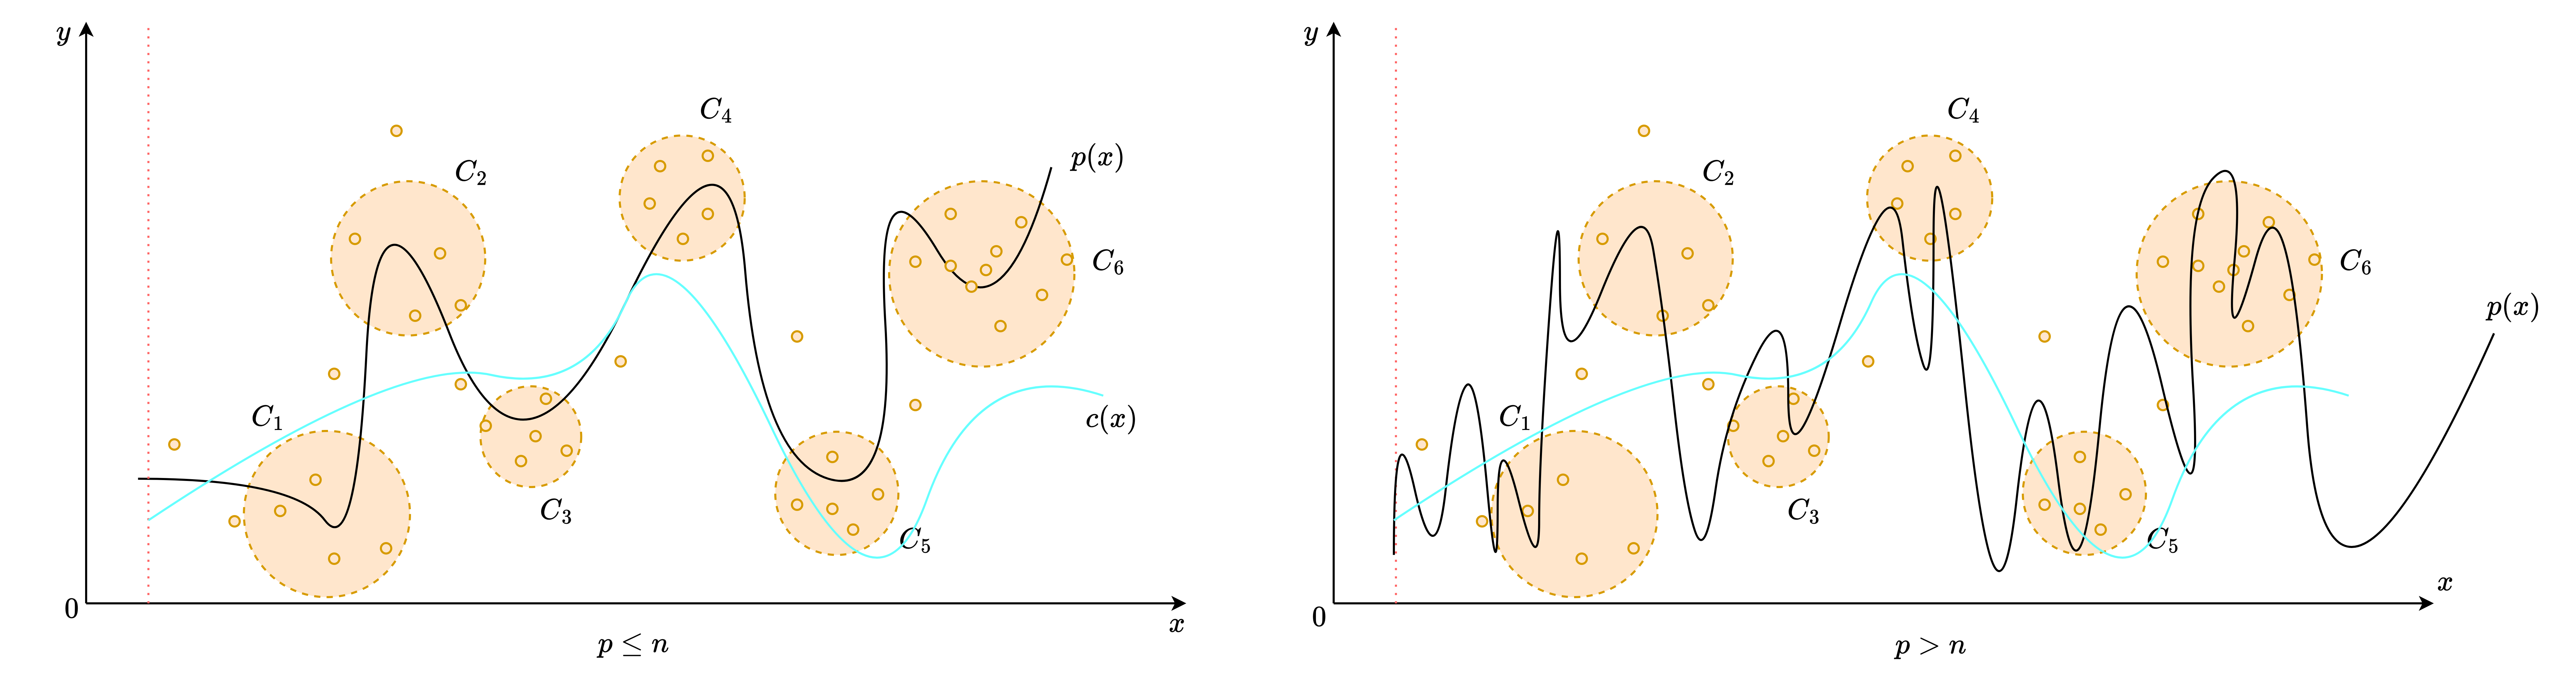
\includegraphics[width=0.7\textwidth]{media/diagram_poly_dd.png}
  \caption{\small\textbf{Intuition of Hypothesis~\ref{hyp:hypothesis_poly_dd}}. Effectively, in the overparameterized range $(p>n)$, the problem turns into soft interpolation, where the polynomial is possible to be dense enough such that relative error remains internally low. This can also happen if the dataset itself is intrinsically large.}
\end{figure}

That is, the disparity between the test and training dataset helps in such regard. If the two dataset is partitioned in the sense that their deviation is practically the same (which can be done using synthetic generation for a control group), then this will amount to not much of it. After all, it will be the consequence of the algorithm and error landscape interpretation used. 

For this, we propose another speculative observation beside such, as to consider adjourned transform of the Vandermonde basis to the Newtonian or similar basis, in which the effects and motion can be easily observed, as least easy. This is because aside from mapping down to $[-1,1]$, normal polynomial on monomial basis gives suboptimal result because of intrinsic high-degree term domination. This will become more relevant later on in the analysis. 